\documentclass[12pt, dvipdfmx]{beamer}

\renewcommand{\kanjifamilydefault}{\gtdefault}
%%%%%%%%%%%  package  %%%%%%%%%%%
\usepackage{bxdpx-beamer}% dvipdfmxなので必要
\usepackage{pxjahyper}% 日本語で'しおり'したい

\usepackage{amssymb,amsmath,ascmac}

\usepackage{multirow}
\usepackage{bm}

\graphicspath{{../../../_Figures//}{../../../_Figures/gakkai/}{./}}

\usepackage{tikz}
\usepackage{xparse}

\usepackage{multimedia}

\usetikzlibrary{shapes,arrows}
%% define fancy arrow. \tikzfancyarrow[<option>]{<text>}. ex: \tikzfancyarrow[fill=red!5]{hoge}
\tikzset{arrowstyle/.style n args={2}{inner ysep=0.1ex, inner xsep=0.5em, minimum height=2em, draw=#2, fill=black!20, font=\sffamily\bfseries, single arrow, single arrow head extend=0.4em, #1,}}
\NewDocumentCommand{\tikzfancyarrow}{O{fill=black!20} O{none}  m}{
\tikz[baseline=-0.5ex]\node [arrowstyle={#1}{#2}] {#3 \mathstrut};}

%微分関連のマクロ
%
\newcommand{\diff}{\mathrm d}
\newcommand{\difd}[2]{\dfrac{\diff #1}{\diff #2}}
\newcommand{\difp}[2]{\dfrac{\partial #1}{\partial #2}}
\newcommand{\difdd}[2]{\dfrac{\diff^2 #1}{\diff #2^2}}
\newcommand{\difpp}[2]{\dfrac{\partial^2 #1}{\partial #2^2}}

%目次スライド
\AtBeginSection[]{
  \frame{\tableofcontents[currentsection]}
}

%アペンディックスのページ番号除去
\newcommand{\backupbegin}{
   \newcounter{framenumberappendix}
   \setcounter{framenumberappendix}{\value{framenumber}}
}
\newcommand{\backupend}{
   \addtocounter{framenumberappendix}{-\value{framenumber}}
   \addtocounter{framenumber}{\value{framenumberappendix}} 
}

\newcommand{\rmd}{\mathrm{d}}
\newcommand{\dd}[1]{\dfrac{\mathrm{d} #1}{\mathrm{d} x}}

%%%%%%%%%%%  theme  %%%%%%%%%%%
\usetheme{Copenhagen}
% \usetheme{Metropolis}
% \usetheme{CambridgeUS}
% \usetheme{Berlin}

%%%%%%%%%%%  inner theme  %%%%%%%%%%%
% \useinnertheme{default}

% %%%%%%%%%%%  outer theme  %%%%%%%%%%%
\useoutertheme{default}
% \useoutertheme{infolines}

%%%%%%%%%%%  color theme  %%%%%%%%%%%
%\usecolortheme{structure}

%%%%%%%%%%%  font theme  %%%%%%%%%%%
\usefonttheme{professionalfonts}
%\usefonttheme{default}

%%%%%%%%%%%  degree of transparency  %%%%%%%%%%%
%\setbeamercovered{transparent=30}

% \setbeamertemplate{items}[default]

%%%%%%%%%%%  numbering  %%%%%%%%%%%
% \setbeamertemplate{numbered}
\setbeamertemplate{navigation symbols}{}
\setbeamertemplate{footline}[frame number]

%%%%%%%%%%%%%%%%%%%%%%%%%%%%%%%%%%%
\title
[ランダムな接続性を有するネットワークポリマーの緩和挙動]
{ランダムな接続性を有する\\ネットワークポリマーの緩和挙動}
\author[東亞合成 佐々木]{佐々木裕}
\institute[東亞合成]{東亞合成}
\date{November 5, 2020}
%%%%%%%%%%%%%%%%%%%%%%%%%%%%%%%%%%
\begin{document}
%%%%%%%%%%%%%%%%%%%%%%%%%%%%%%%%%%
\begin{frame}\frametitle{}
	\titlepage
\end{frame}
% %%%%%%%%%%%%%%%%%%%%%
% \section*{}
% %
% \begin{frame}
% %[allowframebreaks]
% {Outline}
% 	\tableofcontents
% \end{frame}

%%%%%%%%%%%%%%%%%%%%%
\section{はじめに}
%%%%%%%%%%%%%%%%%%%%%%%%%%%%%%%%%%%%%%%%%%%%%
\subsection{本研究の目標とアプローチ}
\begin{frame}
    \frametitle{本研究の目標とアプローチ}
        \begin{block}{目標}
                \begin{itemize}
                    \item 高分子材料の破壊耐性向上の設計指針を得たい。
                    \item 耐久性、可逆性に優れた材料としてゴム材料を選択
                \end{itemize}
        \end{block}
		\begin{exampleblock}{アプローチ}
            \begin{itemize}
                \item 実験的アプローチ
                \begin{itemize}
                    \item 構造明確な\alert{三分岐}ネットワークを超分子で構築
                    \item フィラー無添加での\alert{高い破断伸びと強度}
                    \item 既知のモデルとの多数の整合点と、\alert{よくわからない点}。
                \end{itemize}
                \item マルチスケールシミュレーションで\color{red}モデル\color{black}を構築
                \begin{itemize}
                    \item 単純化したモデルで小さなスケールから始めたい。
                    \item \alert{長さの揃ったストランドで MD シミュレーション}
                    % \item 最終的に、亀裂先端の挙動を FEM シミュレーション
                \end{itemize}
            \end{itemize}
		\end{exampleblock}
\end{frame}

\begin{frame}
	\frametitle{ゴムの強靭性}
	\vspace{-3mm}
		\begin{columns}[totalwidth=\textwidth]
			\column{.48\textwidth}
				\begin{exampleblock}{破壊工学的な考え方}
					\begin{itemize}
						\item クラックの進展を\alert{抑制}
						\item Andrews 理論\footnote{
							\scriptsize
				{Andrews, E. H. and Fukahori, Y. \\J. of Mat. Sci. 12, 1307 (1977)}
						}
							\begin{itemize}
								\item クラックの応力場
								\item クラック進展時に、{\color{red} エネルギー散逸}
								\item \alert{ヒステリシスに由来}
							\end{itemize}	
					\end{itemize}
					% 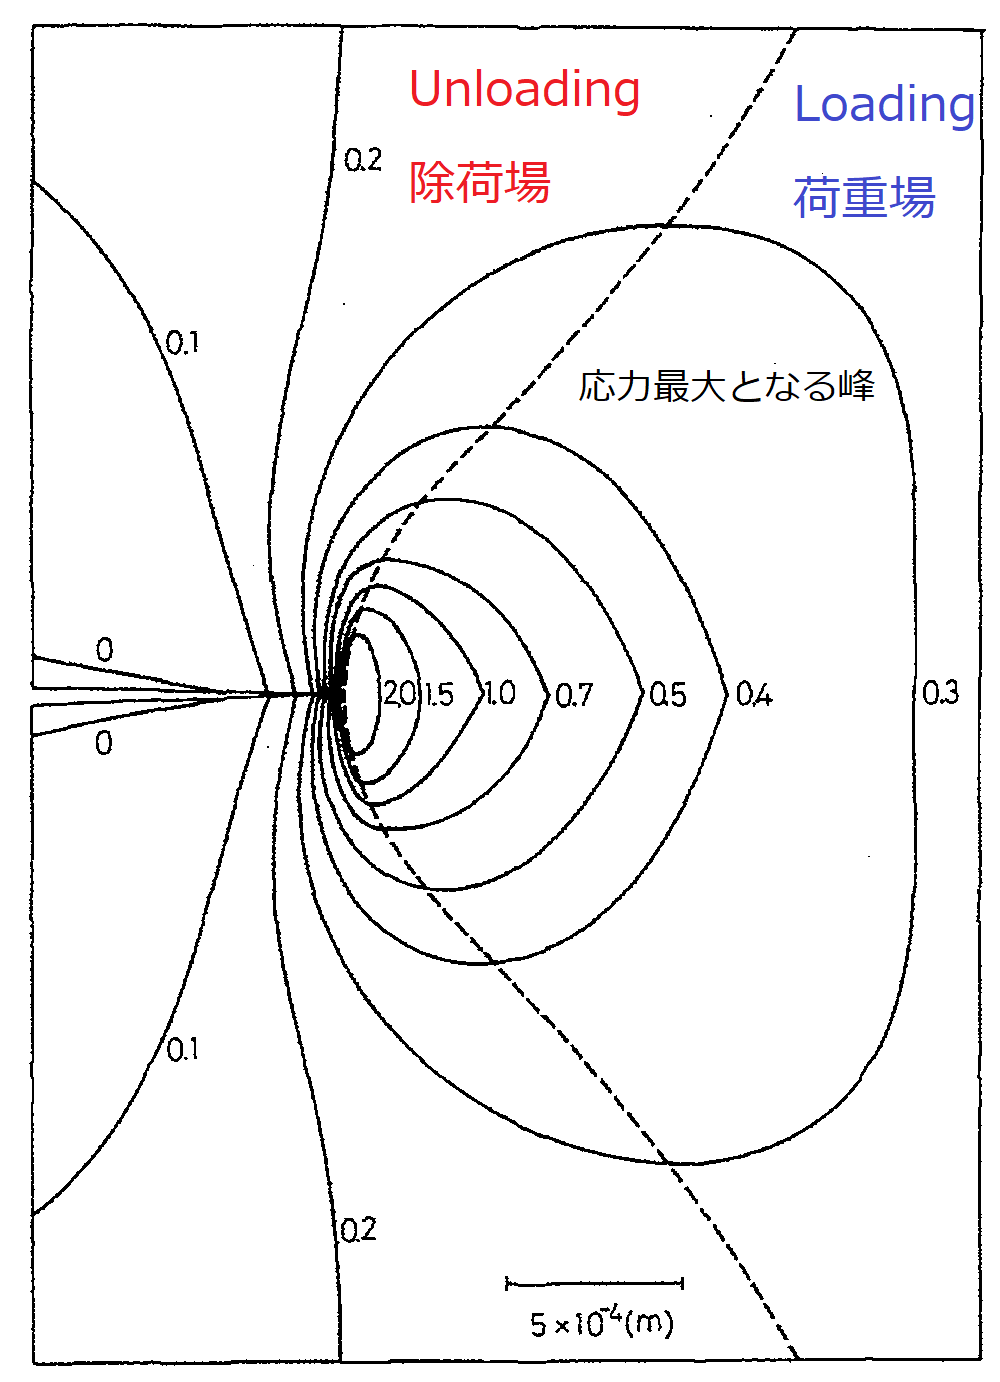
\includegraphics[width=.4\textwidth]{crack.png}
				\end{exampleblock}
				
		\column{.48\textwidth}
		% 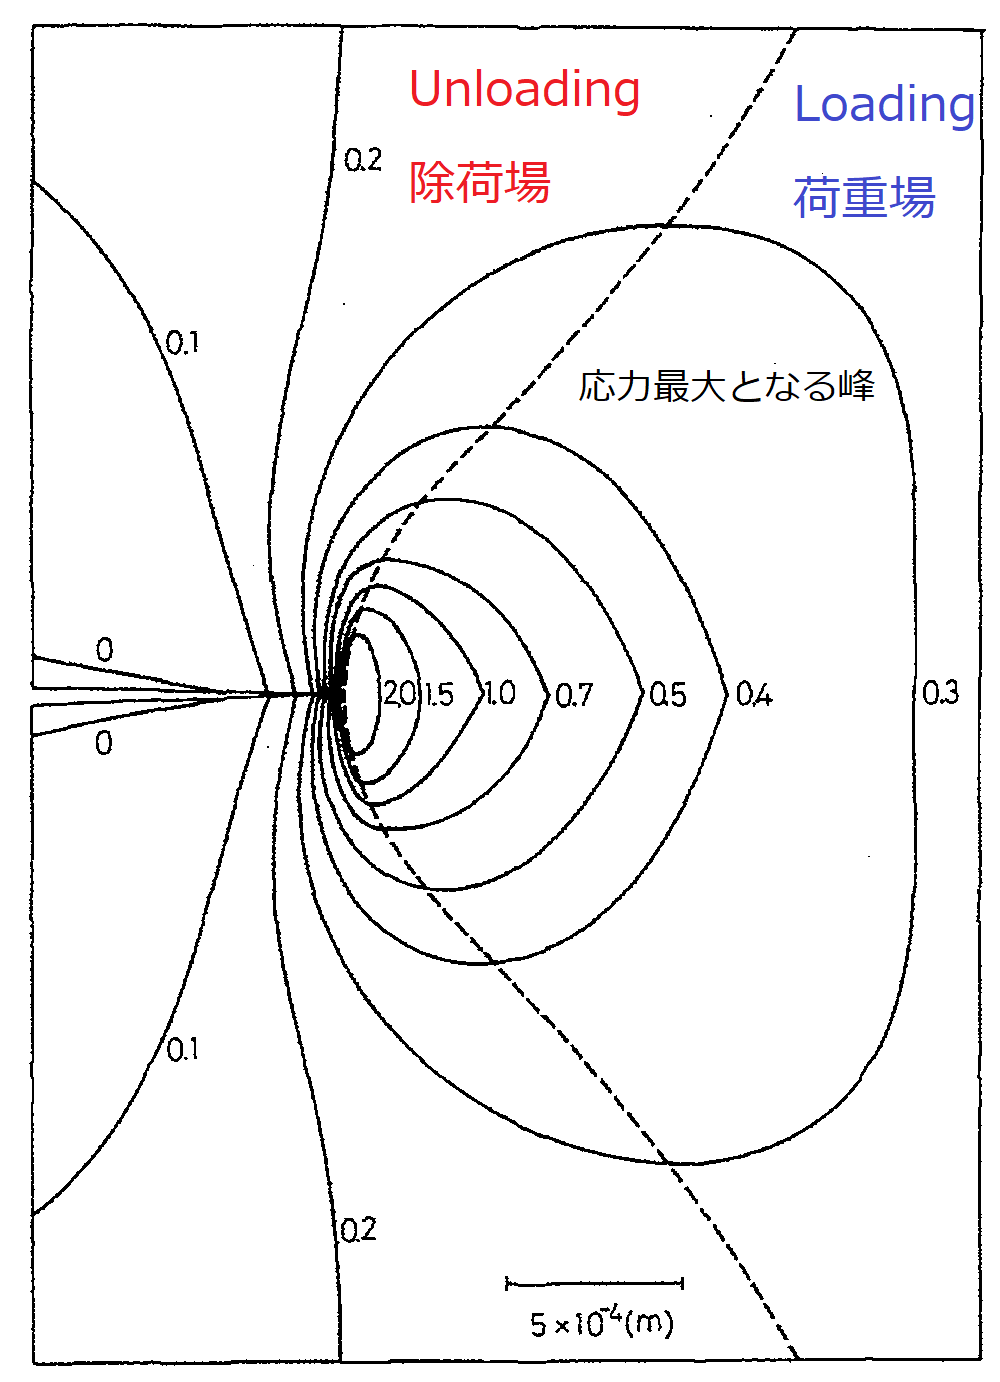
\includegraphics[width=\textwidth]{crack.png}
			\begin{block}{ヒステリシスについて}
				\begin{itemize}
					\item 発生の起源と効果
					\begin{itemize}
						\item フィラーの添加効果\footnote{
							\scriptsize{K. A. Grosch et al. \\Rub. Chem. and Tech.41, 1157 (1968)}
						}
						\item フィラー近傍での\\ナノキャビティーの\\開閉\footnote{
							\scriptsize{H. Zhang et al. \\Macromolecules 46, 900 (2013)}
						}
					\end{itemize}
				\end{itemize}
			\end{block}
		\end{columns}
		\begin{alertblock}{疲労破壊も考慮すると}
			\begin{itemize}
				\item \alert{可逆的}であることが望ましい。\textcolor{blue}{$\neq$ 犠牲結合}
				\item 変形の周期に対応できるように、\alert{回復速度}も重要。
			\end{itemize}
		\end{alertblock}
\end{frame}

\begin{frame}
    \frametitle{古典ゴム弾性理論}
        \vspace{-6mm}
        \begin{columns}[T, onlytextwidth]
            \column{.48\linewidth}
                \begin{block}{ひずみ不変量に対して}
                    \begin{itemize}
                        \item 自由エネルギー密度変化の一般式
                        \vspace{-3mm}
                        \scriptsize
                        \begin{align*}
                            \dfrac{F}{V} &= \sum_{i,j = 0}^{\infty} C_{ij}(I_1-3)^i(I_2-3)^j \\
                            &= C_0 + C_1 (I_1-3) + C_2(I_2-3) \\
                            &\;\;\;\;\;+ \sum_{i,j = 1}^{\infty} C_{ij}(I_1-3)^i(I_2-3)^j
                        \end{align*}
                        \normalsize
                        \item Mooney-Rivlin の式
                        \vspace{-3mm}
                        \scriptsize
                        \begin{align*}
                            \dfrac{F}{V} &= C_1 (I_1-3) + C_2(I_2-3)
                        \end{align*}
                        \normalsize
                        \item Neo-Hookean 固体
                        \vspace{-3mm}
                        \scriptsize
                        \begin{align*}
                            \dfrac{F}{V} &= C_1 (I_1-3)
                        \end{align*}
                        \normalsize
                    \end{itemize}
                \end{block}
            \column{.48\linewidth}
                \begin{exampleblock}{ミクロな変形モデル}
                    Neo-Hookean 固体の\\一軸伸張では、
                    \begin{itemize}
                        \item Affine Network Model
                            \begin{itemize}
                                \item アフィン変形を仮定
                            \end{itemize}
                            \vspace{-3mm}
                            \scriptsize
                            \begin{align*}
                                \sigma_{nom} &= \textcolor{red}{\nu} k_B T \left(\lambda - \dfrac{1}{\lambda^2}\right) \\
                                &= G_{affine} \left(\lambda - \dfrac{1}{\lambda^2}\right)
                            \end{align*}
                            \normalsize
                        \item Phantom Network Model
                        \vspace{-5mm}
                            \begin{itemize}
                                \item \alert{架橋点ゆらぎ}を考慮
                                \item 架橋点の分岐数 $f$
                            \end{itemize}
                            \vspace{-3mm}
                            \scriptsize
                            \begin{align*}
                                G_{phantom} &= \nu k_B T \left(1 - \dfrac{2}{f}\right) \\
                            \end{align*}
                            \normalsize
                    \end{itemize}
                \end{exampleblock}
        \end{columns}       
\end{frame}


\subsection{これまでの検討結果}
\begin{frame}
	\frametitle{規則ネットワーク構造MDシミュレーション}
	\begin{columns}[totalwidth=1\textwidth]
		\column{.55\textwidth}
			ストランド長一定の規則構造
			\begin{itemize}
				\item 分岐数 
					\begin{itemize}
						\item 三分岐\\K4 構造
						\item 四分岐\\ダイヤモンド構造
					\end{itemize}
				\item ストランド
					\begin{itemize}
						\item KG鎖\\LJ ポテンシャルにより、\alert{排除体積効果}を導入
						\item 素抜け鎖\\長距離相互作用を\\無視した\alert{理想鎖}
					\end{itemize}
			\end{itemize}
		\column{.42\textwidth}
			\begin{itemize}
				\item K4 構造

				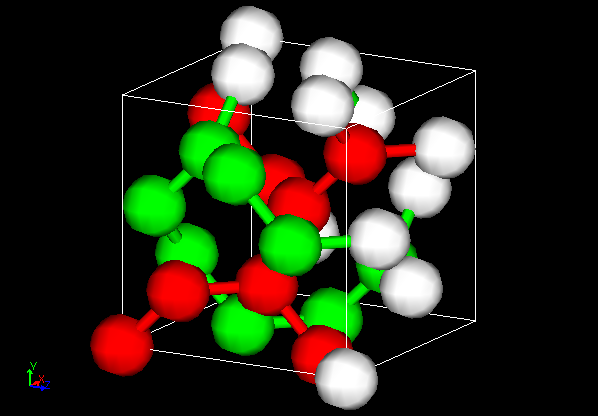
\includegraphics[width=0.8\textwidth]{K4_d.png}

				\item ダイヤモンド構造

				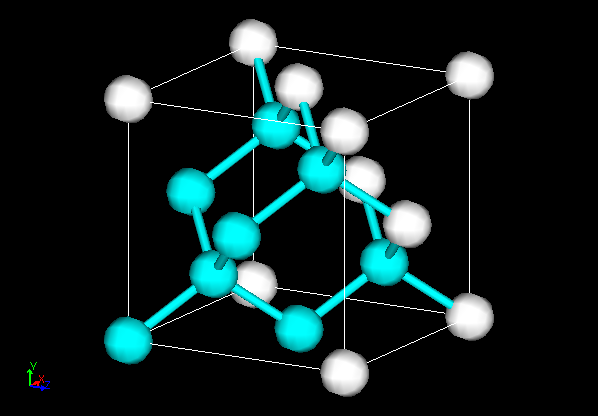
\includegraphics[width=0.8\textwidth]{dia.png}

			\end{itemize}
	\end{columns}
\end{frame}

\begin{frame}
	\frametitle{規則ネットワーク構造での検討結果}
		\small
		\begin{alertblock}{規則ネットワーク構造の振る舞い}
			\begin{itemize}
				\item 一軸伸長で、\alert{アフィンネットワークモデルの挙動}を示した
					\begin{itemize}
						\item \alert{分岐数、ストランドの性質(KG、素抜け)}によらず
				%	\item
				%	伸びきり効果をほぼ再現
					\end{itemize}
				\item 応力緩和で、主緩和が\alert{ラウスモードの最長緩和時間}程度
				\item 主緩和近傍に\alert{大きなエネルギー散逸($\tan \delta > 1$)}を確認
			\end{itemize}
		\end{alertblock}
		\begin{columns}[totalwidth=1\textwidth]
			\column{.32\textwidth}
				\scriptsize
				一軸伸長結果
				% \vspace{-2mm}
				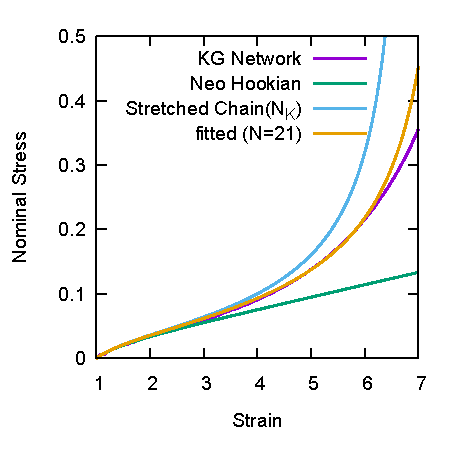
\includegraphics[width=0.9\textwidth]{SS_Kuhn.pdf}
			\column{.32\textwidth}
				\scriptsize
				応力緩和挙動
				% \vspace{-2mm}
				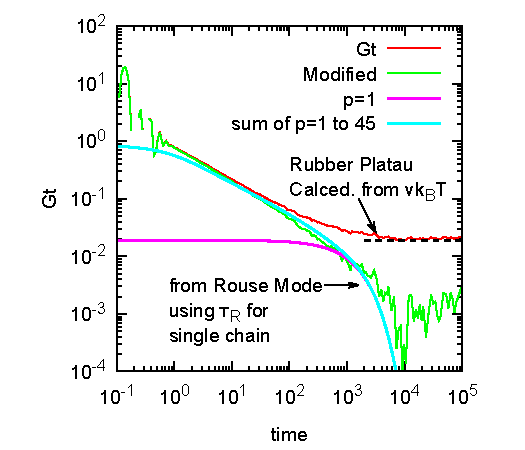
\includegraphics[width=0.9\textwidth]{Gt_loglog.pdf}
			\column{.32\textwidth}
				\scriptsize
				粘弾性スペクトル
				% \vspace{-2mm}
				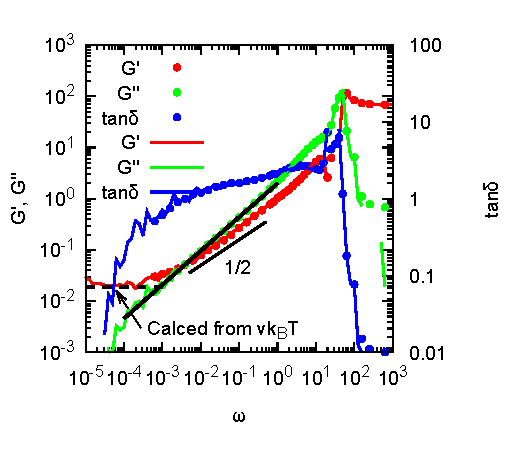
\includegraphics[width=\textwidth]{N_44_Freq_Sweep.pdf}
		\end{columns}
\end{frame}

\begin{frame}
	\frametitle{規則構造でのアフィン性}
		\begin{columns}[totalwidth=\linewidth]
			\column{.5\linewidth}
				\begin{block}{規則構造の特徴}
					\begin{itemize}
						\item 規則構造においては、\\結節点の\alert{連結性は等価}
							\begin{itemize}
								% \item それぞれの結節点の\\ゆらぎも等価
								\item 結節点は規則構造の\\平均位置に拘束
							\end{itemize}
						\item 巨視的な変形後
							\begin{itemize}
								\item 結節点の\alert{平均位置が\\アフィン移動}
								\item ゆらぎの異方性も類似
							\end{itemize}
					\end{itemize}
				\end{block}
			\column{.45\linewidth}
				規則構造の模式図
				\vspace{3mm}
				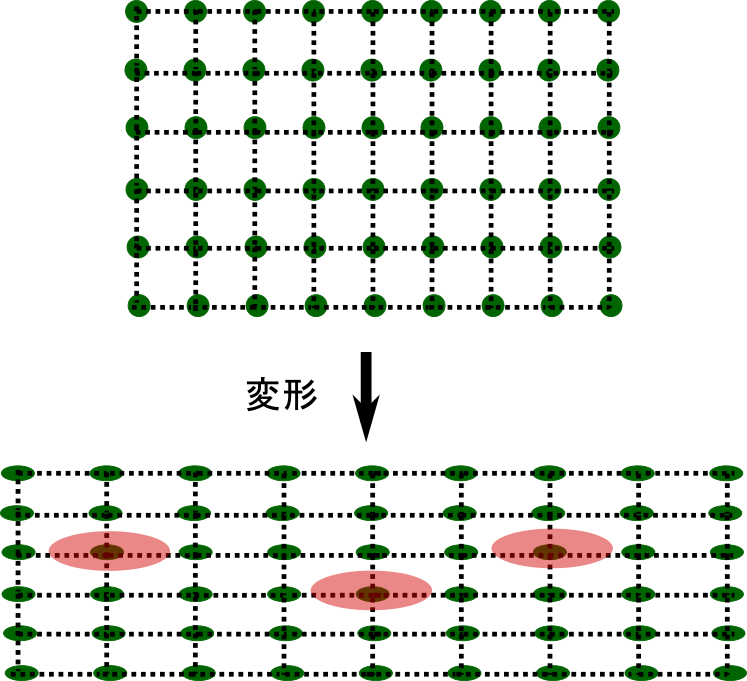
\includegraphics[width=\columnwidth]{reglar_NW_2.png}
		\end{columns}
		% \begin{center}
		% 	\Large
		% 	\alert{緩和モードも単純}
		% \end{center}
\end{frame}

\begin{frame}
	\frametitle{これまでの検討で出来ていないこと}
		\begin{alertblock}{規則構造でのシミュレーションでは}
			\begin{itemize}
				\item アフィンネットワークモデルでの単純な緩和挙動 
				\begin{itemize}
					\item ガラス転移終端近傍に主緩和
					% \item ゆらぎの異方性が少ないためか?
				\end{itemize}
			\end{itemize}
		\end{alertblock}
		\begin{block}{ランダムネットワークの検討}
			\begin{itemize}
				\item ネットワーク構造の連結性にランダム性を導入
                    \begin{itemize}
						\item Flory のファントムネットワークの要件に合致
					\end{itemize}
				\item ランダムネットワークモデルの特徴
				\begin{itemize}
					\item アフィン変形を抑制?
					\item 架橋点のゆらぎに起因した多様な緩和モードが発現?
					\item 緩和強度の増大、あるいは、長時間化?
				\end{itemize}
			\end{itemize}
		\end{block}
\end{frame}

\begin{frame}
    \frametitle{ランダム性の導入}
    \vspace{-3mm}
		\begin{columns}[totalwidth=1\textwidth]
			\column{.45\textwidth}
				\begin{block}{連結のランダム性を導入}
					\begin{itemize}
						\item 連結性を不均一に
							\begin{itemize}
								\item 連結に\alert{位置依存性}
							\end{itemize}
						\item 巨視的な変形後
							\begin{itemize}
								\item 結節点のゆらぎが\\不均一
								\item 多様な緩和モード
								\item \alert{緩和の長時間化?}
							% \item ファントムネットワークモデルの諸特性の発現?
							\end{itemize}
						\item \alert{解析を容易}に、
                            \begin{itemize}
                                \item 既往研究で反応系
								\item ストランド長と\\結合数を一定
							\end{itemize}
					\end{itemize}
				\end{block}
			\column{.52\textwidth}
				ランダム構造の模式図
				\vspace{5mm}
				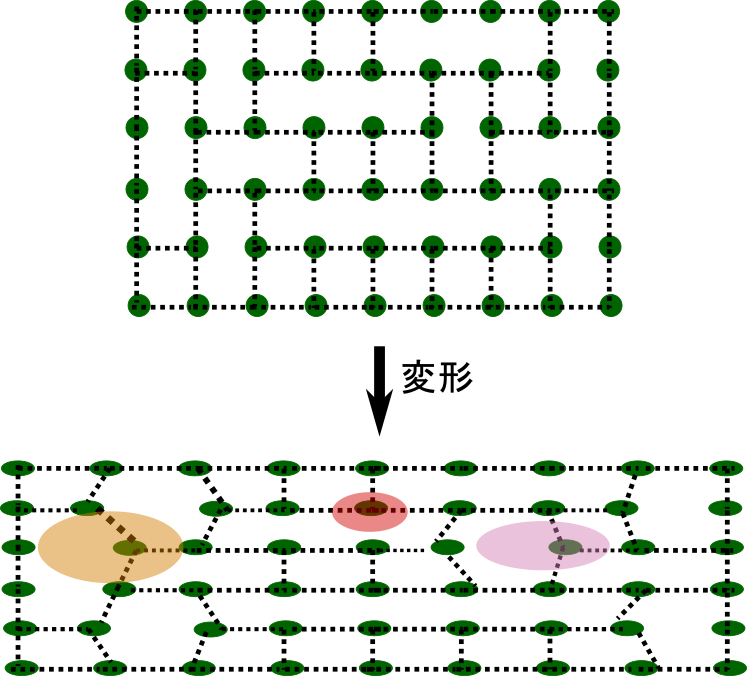
\includegraphics[width=\textwidth]{random_NW.png}
    \end{columns}
    \vspace{-3mm}
	\begin{center}
		\begin{alertblock}<2>{}
			\alert{「素抜け鎖」でのランダムネットワークはすでに報告。}
		\end{alertblock}
	\end{center}
\end{frame}

\subsection{本発表の内容}
\begin{frame}
	\frametitle{本発表の内容}
		\begin{block}{素抜け鎖のランダムネットワーク}
			\begin{itemize}
				\item ランダムネットワーク作成のプロセス
				\item ネットワークの力学的応答
				\begin{itemize}
					\item \alert{ファントムネットワークモデル}を確認
				\end{itemize}
			\end{itemize}
		\end{block}
		\begin{alertblock}{KG 鎖のランダムネットワークでの検討}
			\begin{itemize}
				\item KG鎖の初期構造緩和
				\item 力学的及び緩和挙動の明確化。
				\item 絡み合いの影響を確認
				\begin{itemize}
					\item PPA での絡み合いの可視化
					\item Z1-code による比較
				\end{itemize}
			\end{itemize}
		\end{alertblock}
\end{frame}


\section{「素抜け鎖」のランダムネットワークシミュレーション}
\subsection{ランダムネットワーク作成のアルゴリズム}
\begin{frame}
	\frametitle{ランダムなネットワークの作成}
		\begin{exampleblock}{アルゴリズム}
			\begin{enumerate}
				\item 初期構造の作成
					\begin{itemize}
						\item \alert{実空間}で8-Chain Model で初期構造を作成。
						\item 所望の分岐数に\alert{ランダム}に選択した\alert{結合を除去}
						\item 除去したジオメトリーに対応した\alert{トポロジーモデル}
					\end{itemize}
				\item トポロジー空間でランダム性の導入
					\begin{itemize}
						\item ラプラシアン行列で全体の連結性を確認しながら、
						\item \alert{エッジ交換}して、ランダム性を導入
					\end{itemize}	
				\item 対応する\alert{実空間でのネットワーク初期構造}を作成
			\end{enumerate}
		\end{exampleblock}
		\begin{columns}[T, onlytextwidth]
			\column{.33\linewidth}
				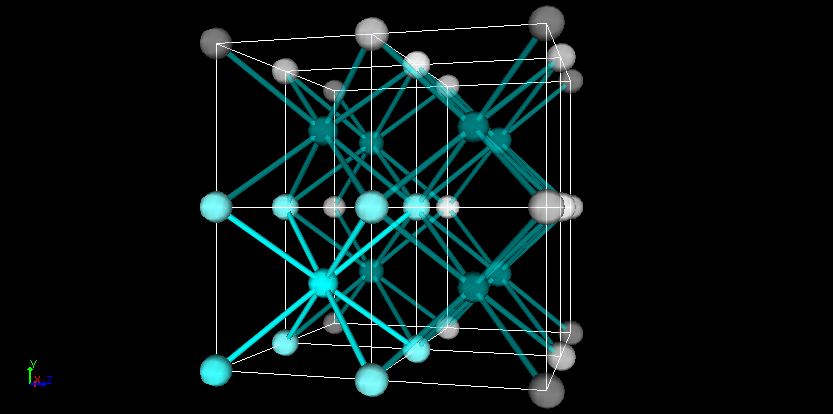
\includegraphics[width=\textwidth]{8_per.png}
			\column{.33\linewidth}
				\vspace{-5mm}
				\begin{center}
					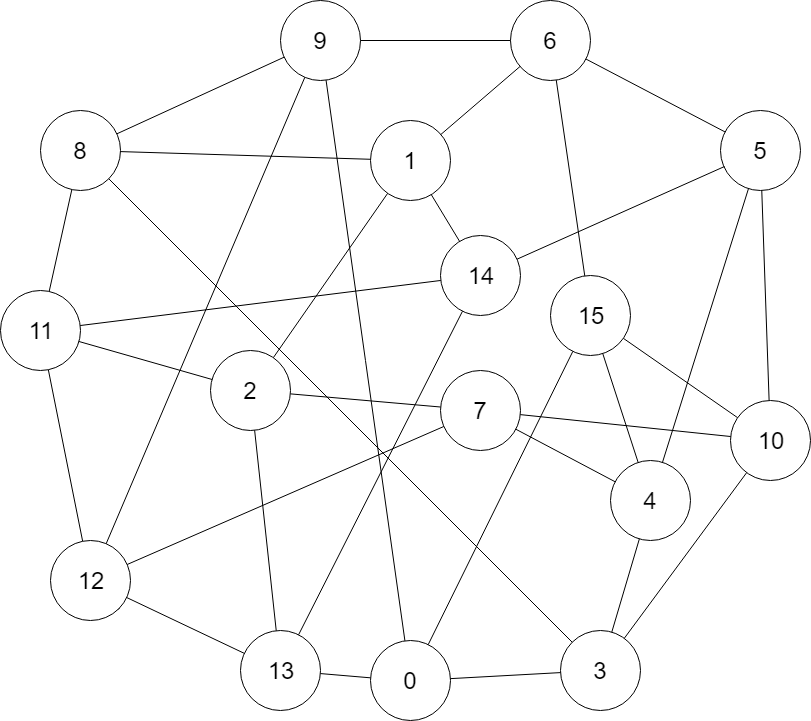
\includegraphics[width=.65\textwidth]{Network.png}
				\end{center}
			\column{.33\linewidth}
				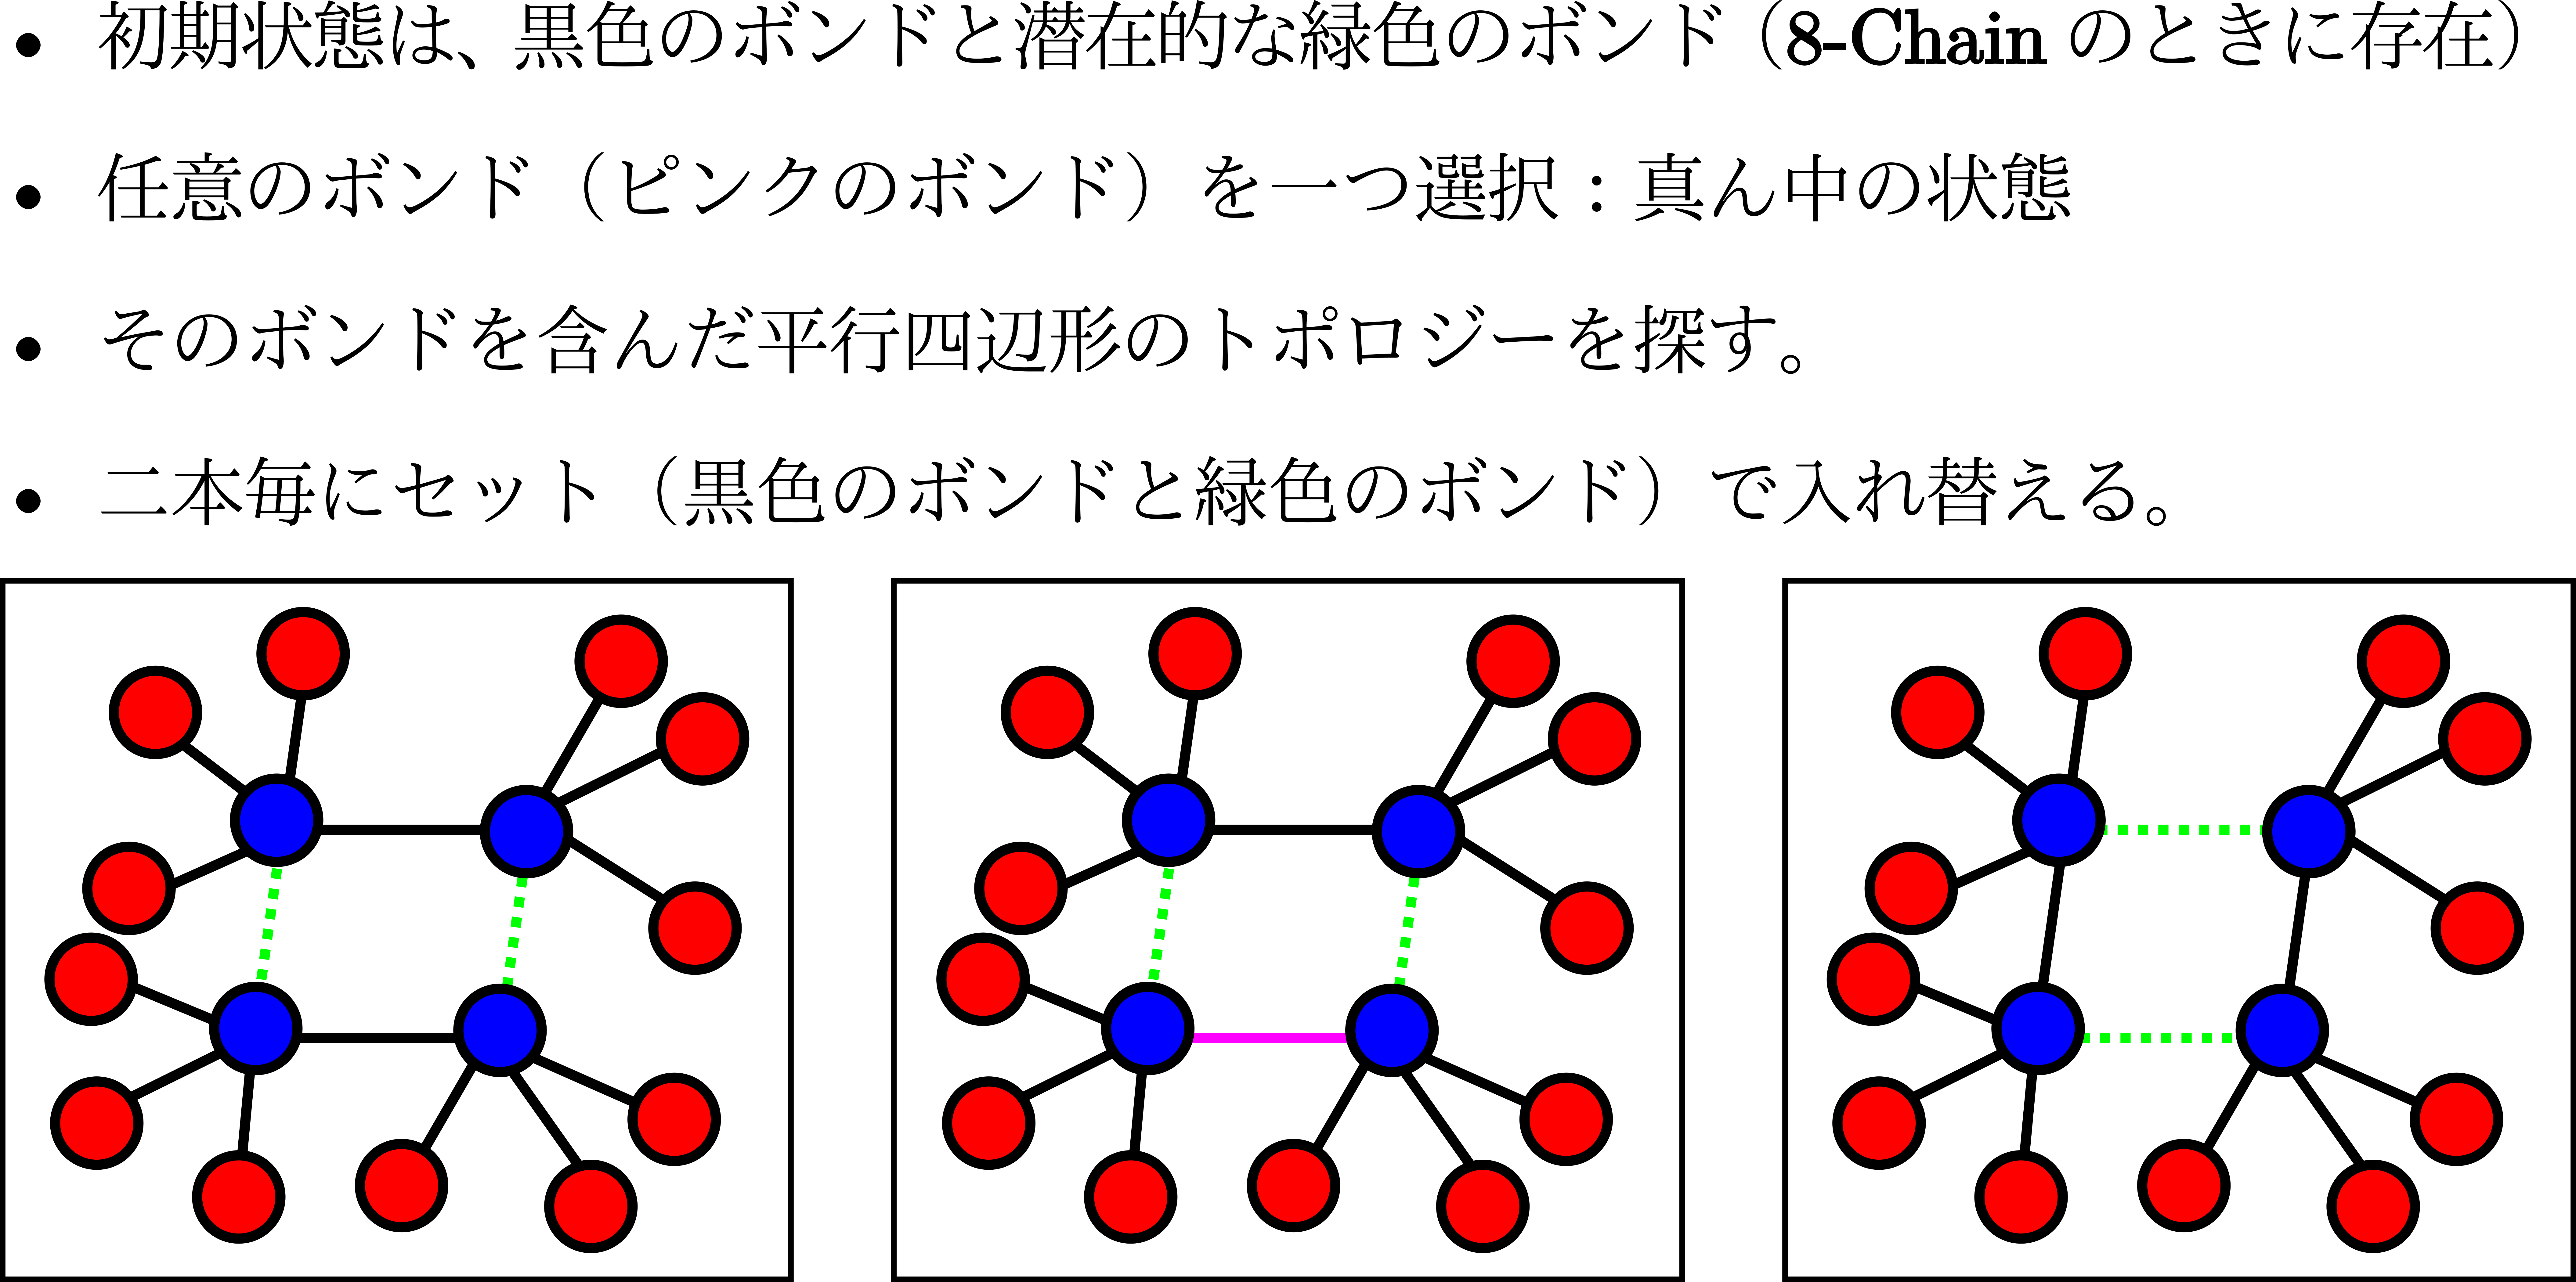
\includegraphics[width=\textwidth]{bond_exchg.png}
		\end{columns}
\end{frame}

\subsection{「素抜け鎖」のシミュレーション結果}
\begin{frame}
	\frametitle{「素抜け鎖」の力学応答}
		\begin{alertblock}{「素抜け鎖」でのランダムネットワーク}
			\begin{itemize}
				% \item ストランド:す抜け鎖
				\item 四分岐ランダムネットワークモデル
			\end{itemize}
        \end{alertblock}
        \vspace{-3mm}
		\begin{columns}[totalwidth=\linewidth]
			\column{.48\linewidth}
				\begin{block}{一軸伸張結果}
					\begin{itemize}
						\item 伸張速度低下で\alert{ファントム応答}に漸近
						% \item 低伸張率から伸び切り
                    \end{itemize}
                    \begin{center}
                        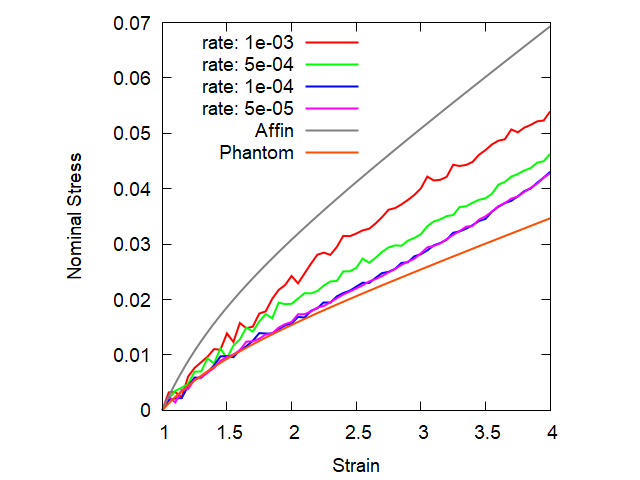
\includegraphics[width=.9\columnwidth]{N48_sunuke.png}
                    \end{center}
				\end{block}
			\column{.48\linewidth}
				\begin{exampleblock}{ステップ変形の応力緩和}
                    \begin{itemize}
                        \item 高速伸長:$\dot{\gamma} = 1e^{-3}$
                        \item 変位:$\lambda = 1.5$
                    \end{itemize}
					\begin{center}
                        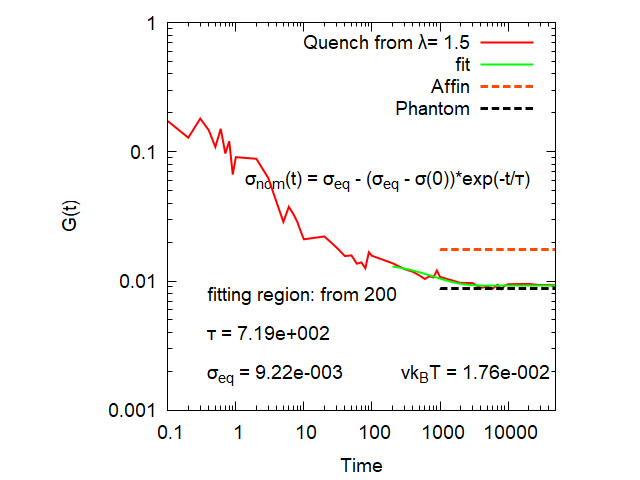
\includegraphics[width=.9\columnwidth]{gt_sunuke.png}
                    \end{center}
				\end{exampleblock}
		\end{columns}
\end{frame}

\section{KG鎖でのシミュレーション結果}
\subsection{初期構造の緩和}
\begin{frame}
    \frametitle{初期構造の緩和}
        \vspace{-2mm}
		\begin{block}{KG 鎖をストランドとするネットワーク}
			\begin{itemize}
				\item KG鎖は「非素抜け」なので、\alert{初期構造の緩和}が重要。
				\vspace{-3mm}
					\fontsize{6pt}{0pt}
					\begin{align*}
						&U_{KG}(r) = 
						\begin{cases}
						U_{nonbond} = U_{LJ} \;\text{where } r_c = 2^{(1/6)}\sigma \\
						U_{bond} = U_{LJ} + U_{FENE}
						\end{cases} 
					\end{align*}
			\end{itemize}
		\end{block}
		\vspace{-3mm}
		\begin{columns}[T, onlytextwidth]
			\column{.66\linewidth}
				\begin{exampleblock}{初期構造の緩和}
					\begin{itemize}
						\item Auhl 等の方法\footnote{
							\scriptsize{R. Auhl et al. J. of Chem. Phys., 119, 12718 (2003)}
						}に従い、
						\begin{itemize}
							\item force-capped-LJ ポテンシャル
							\item Slow Push Off で初期構造を緩和
						\end{itemize}
					\end{itemize}
					\vspace{-3mm}
					\fontsize{6pt}{0pt}
					\begin{align*}
						&U_{FCLJ}(r) = 
						\begin{cases}
						(r-r_{fc})*U_{LJ}^{\prime}(r_{fc}) + U_{LJ}(r_{fc}) \; &r< r_{fc} \\
						U_{LJ}   \;\;\;\;\;\;\; &r \geq r_{fc}
						\end{cases} 
					\end{align*}
				\end{exampleblock}
			\column{.32\linewidth}
				\vspace{2mm}
				\begin{center}
					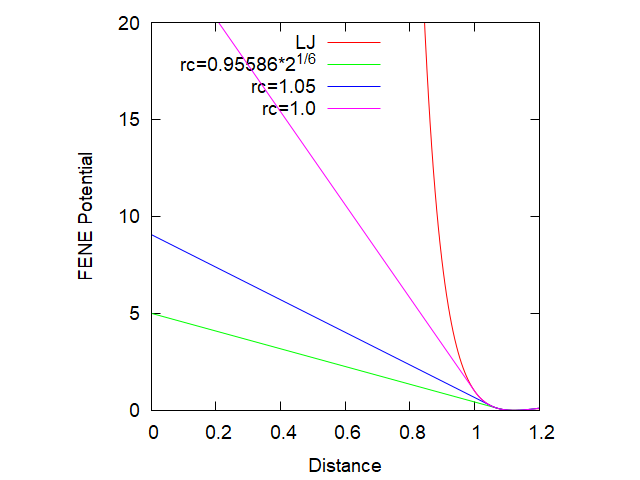
\includegraphics[width=1.2\textwidth]{Ev_fcLJ.png}
				\end{center}
				\vspace{-3mm}
				\scriptsize
				\begin{itemize}
					\item force-capped-LJ Pot.
					\item 素抜け⇒絡み合い
				\end{itemize}
		\end{columns}
\end{frame}

\subsection{力学的な応答}
\begin{frame}
	\frametitle{四分岐ネットワークの力学応答}
		\begin{columns}[T, onlytextwidth]
			\column{.48\linewidth}
				\begin{block}{一軸伸張結果}
					\begin{itemize}
						\item 伸張速度の低下によりネオフッキアンに漸近
						\item ANMよりも応力は高い
					\end{itemize}
					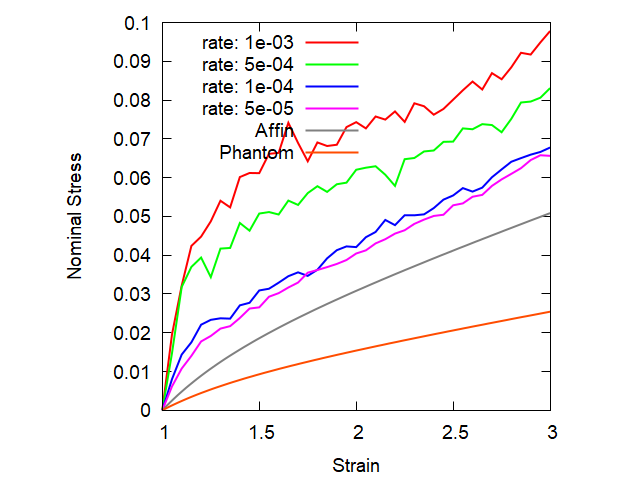
\includegraphics[width=\textwidth]{N48_C4_M3.png}
				\end{block}
				
			\column{.48\linewidth}
				\begin{block}{Moony-Rivlin Plot}
					\begin{itemize}
						\item Shear Rate = 1e-4
						
						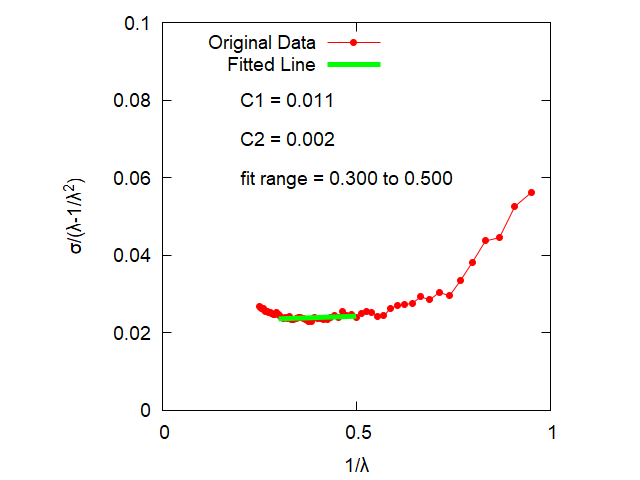
\includegraphics[width= .6\textwidth]{MR_rate_1e-04.png}
						\item Shear Rate = 5e-5
						
						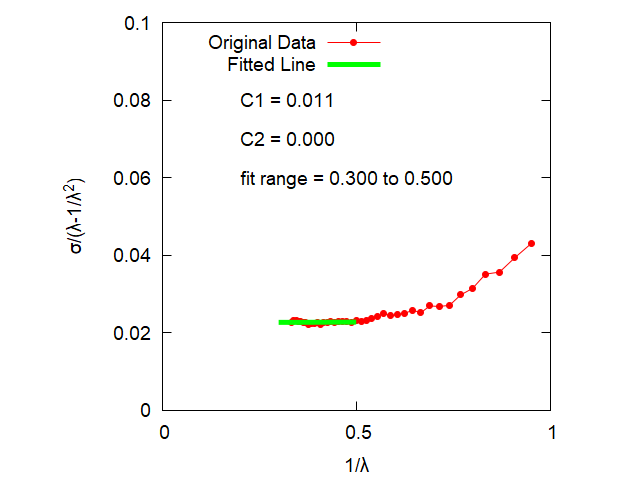
\includegraphics[width= .6\textwidth]{MR_rate_5e-05.png}
					\end{itemize}
					
				\end{block}
		\end{columns}
\end{frame}

\begin{frame}
	\frametitle{四分岐ネットワークの力学応答}
		\begin{columns}[T, onlytextwidth]
			\column{.48\linewidth}
				\begin{block}{一軸伸張結果}
					\begin{itemize}
						\item 伸張速度の低下によりネオフッキアンに漸近
						\item ANMよりも応力は高い
					\end{itemize}
					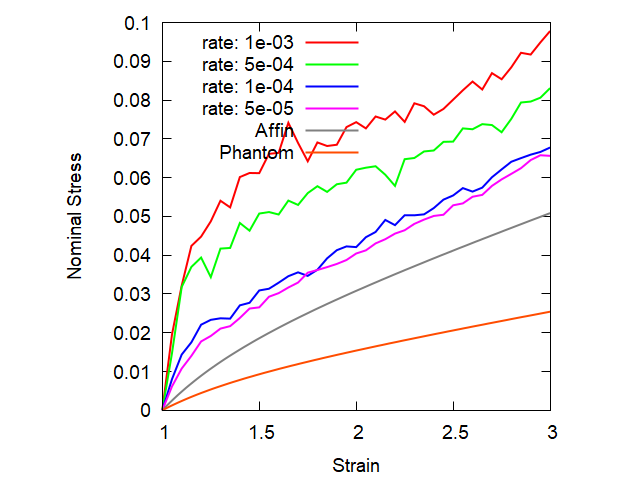
\includegraphics[width=\textwidth]{N48_C4_M3.png}
				\end{block}
				
			\column{.48\linewidth}
				\begin{block}{応力緩和関数 $G(t)$}
					\begin{itemize}
						\item ステップ変形($\lambda=2.0$)
						\item 最長緩和の長時間化
						\item ANM よりも高弾性率
					\end{itemize}
					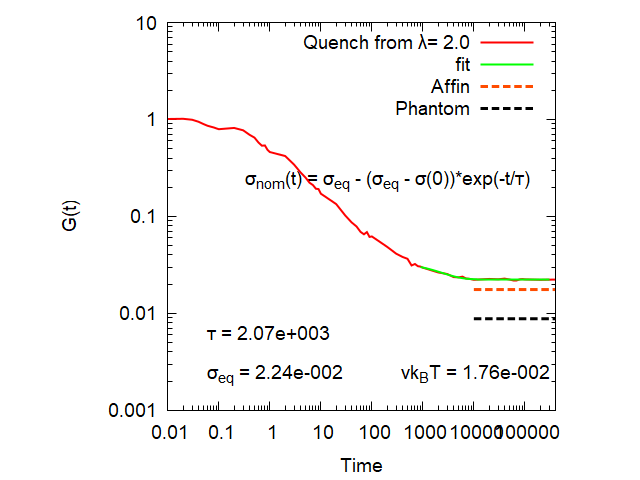
\includegraphics[width=\textwidth]{gt_N48_C4_M3.png}
				\end{block}
		\end{columns}
\end{frame}

\begin{frame}
	\frametitle{ランダムネットワークの絡み合い解析}
		\vspace{-6mm}
		\begin{columns}[T, onlytextwidth]
			\column{.48\linewidth}
			\begin{block}{N48 のネットワークのPPA}
				\begin{itemize}
					\item ストランド内部の非結合ポテンシャルを無効
					\item \alert{多数の絡み合いが存在}
				\end{itemize}
				\begin{center}
					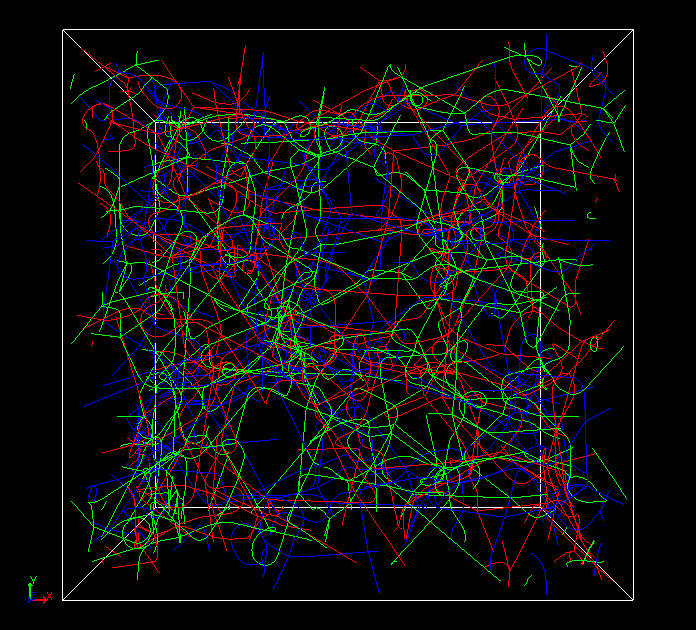
\includegraphics[width=.65\textwidth]{N48_f4_PPA.png}
				\end{center}
				
			\end{block}
			\column{.48\linewidth}
			\begin{block}{仮想的なモデル状態}
				\begin{itemize}
					\item 全ての非結合ポテンシャルを無効
					\item す抜けに設定したPPA
				\end{itemize}
				\begin{center}
					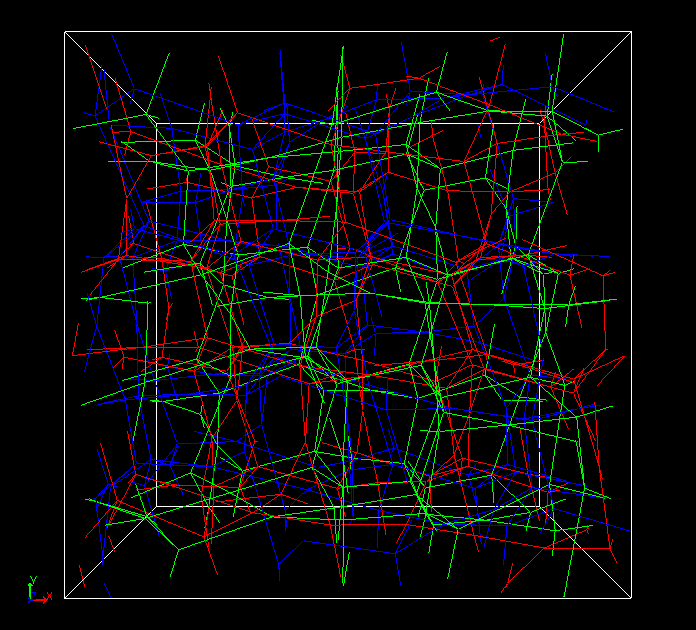
\includegraphics[width=.65\textwidth]{PPA_sunuke_NW.png}
				\end{center}
			\end{block}
		\end{columns}
        \vspace{-2mm}
        \small
		\begin{screen}
			PPA: Primitive Path Analysis\footnote{
                S. K. Sukumaran, et al., J. of Polym. Sci., Part B, 43, 917 (2005)
            }
		\end{screen}
\end{frame}

\begin{frame}
    \frametitle{Z1-code での確認}
        \vspace{-3mm}
        \begin{columns}[T, onlytextwidth]
            \column{.4\linewidth}
                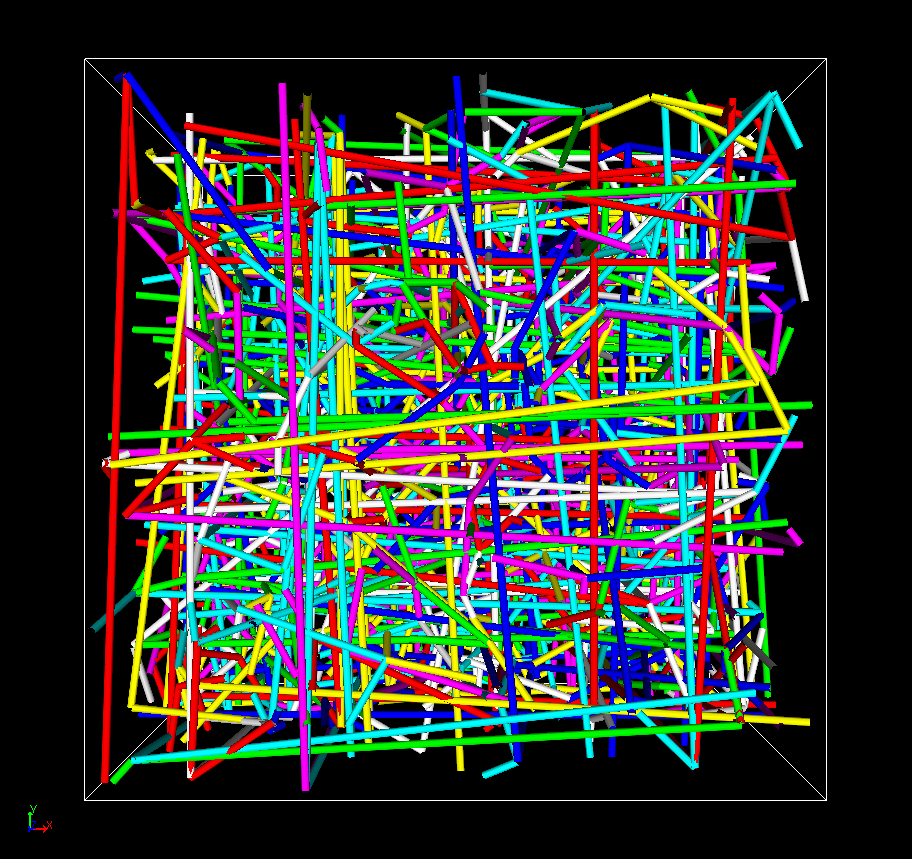
\includegraphics[width=\textwidth]{z_cord_4Chain.png}
                Z1-code での絡み合い
            \column{.56\linewidth}
            \begin{block}{ホモポリマーとの比較}
                \begin{itemize}
                    \item Z は一本鎖あたりの絡み合い
                    \item 今回のネットワークは、\\ホモポリマーと同等
                \end{itemize}
                \scriptsize
                \begin{center}
                    \begin{tabular}{c||c|c} \hline
                        &Homo & 4 Chain NW \\ \hline \hline
                        Segments& 50& 48 \\ \hline
                        Chains & 200& 768 \\ \hline
                        Entanglements& 204& 800\\ \hline
                        Entangled Chains&134&557 \\ \hline
                        \alert{$<Z>_{Z1}$}&\alert{1.02}& \alert{1.04}\\ \hline
                    \end{tabular}
                \end{center}
            \end{block}
        \end{columns}
    \begin{alertblock}{Z1-codeとは}
        \begin{itemize}
            \item 絡み合いを可視化するアルゴリズム\footnote{
                M. Kröger, Comput. Phys. Commun. 168, 209 (2005)
                % \begin{itemize}
                %     \item M. Kröger, Comput. Phys. Commun. 168, 209 (2005)
                %     \item S. Shanbhag, M. Kröger, Macromolecules 40, 2897(2007)
                %     \item R. Hoy, K. Foteinopoulou, M. Kröger, Phys. Rev. E, 31803 (2009)
                % \end{itemize}
            }
        %    N.C. Karayiannis, M. Kröger, Int. J. Mol. Sci. 10, 5054 (2009)
        \end{itemize}
    \end{alertblock}
\end{frame}

\subsection{絡み合いを低減したネットワーク}
\begin{frame}
	\frametitle{絡み合いを低減したネットワーク}
		\begin{exampleblock}{NPT 計算での初期構造の緩和}
			\begin{itemize}
				\item \alert{密度の低い初期状態}から NPT 計算により圧縮して、
				\item 絡み合いを極力排除した初期構造を作成した。
			\end{itemize}
		\end{exampleblock}

		\begin{columns}[T, onlytextwidth]
			\column{.48\linewidth}
				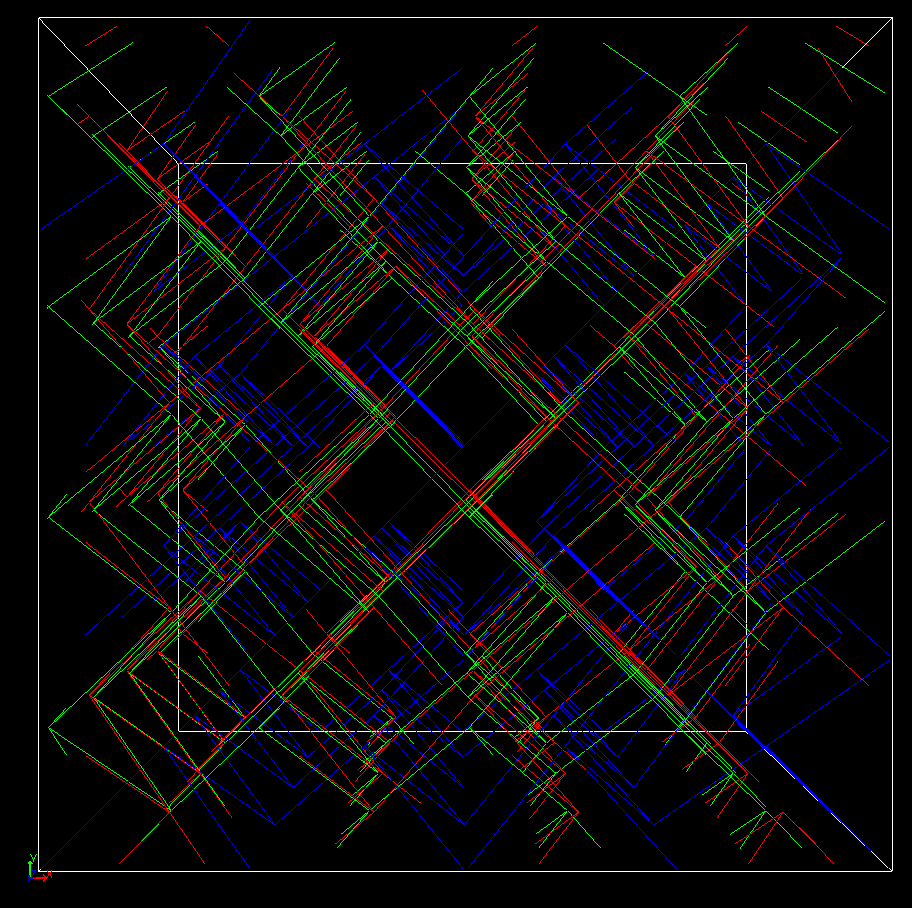
\includegraphics[width=.9\textwidth]{NPT_00.png}
			\column{.48\linewidth}
				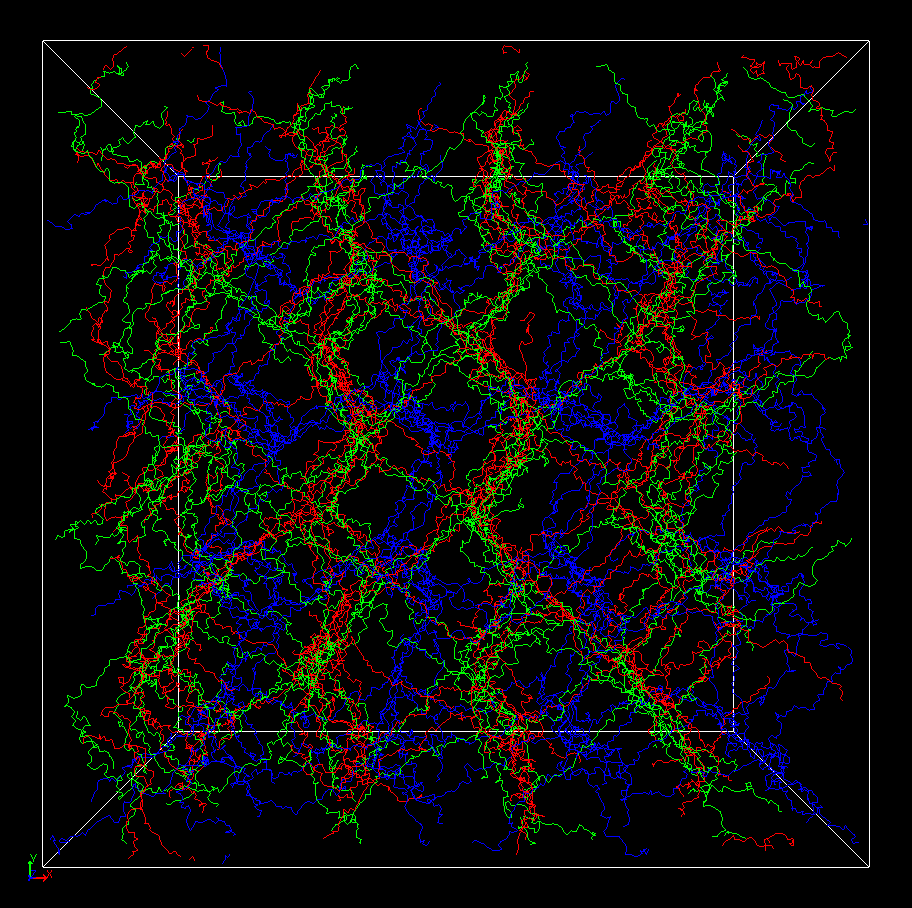
\includegraphics[width=.9\textwidth]{NPT_11.png}
		\end{columns}
\end{frame}

\begin{frame}
    \frametitle{絡み合いを低減したネットワーク}
        \vspace{-3mm}
		\begin{columns}[T, onlytextwidth]
            \column{.45\linewidth}
                \small
				\begin{itemize}
					\item 4-Chain-\alert{NPT}
					
					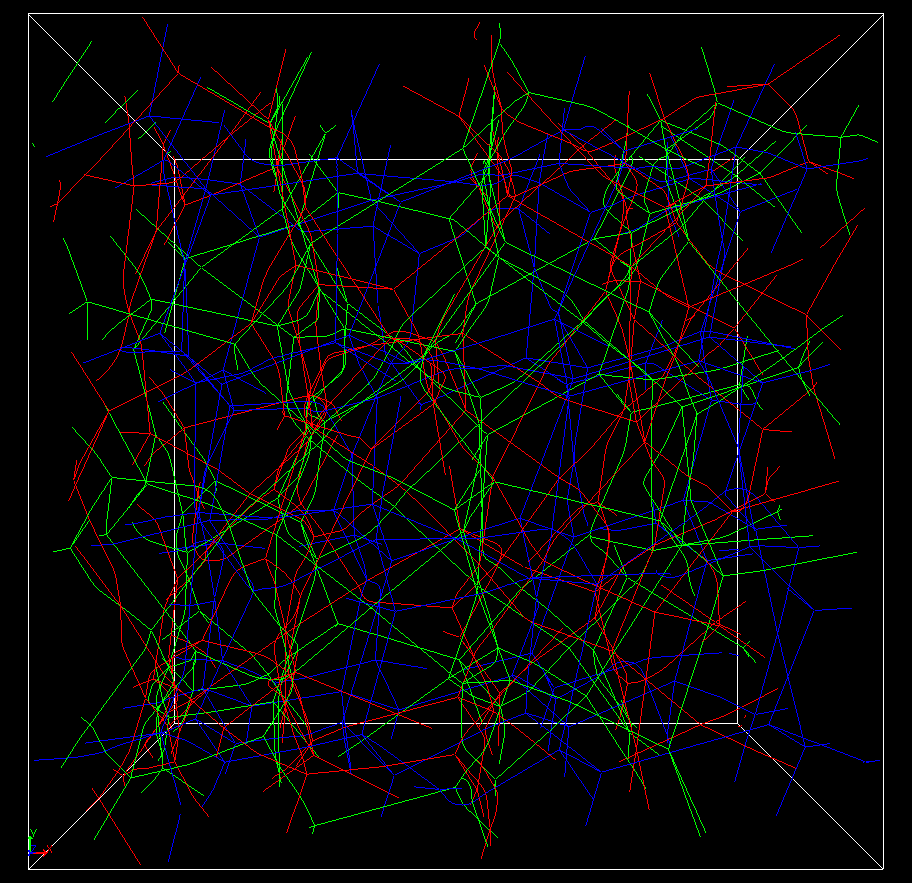
\includegraphics[width=.62\textwidth]{NPT_PPA.png}
					\item 4-Chain-NVT
					
					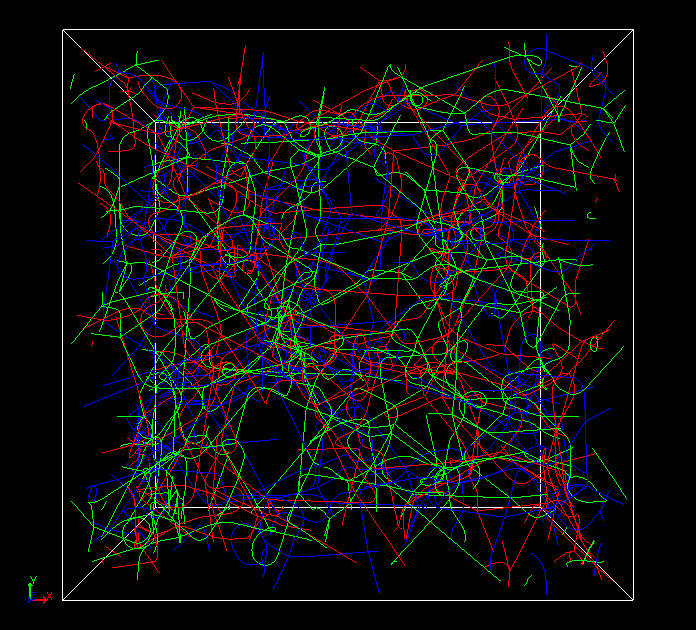
\includegraphics[width=.62\textwidth]{N48_f4_PPA.png}
				\end{itemize}
			\column{.55\linewidth}
			\begin{block}{応力緩和関数 $G(t)$}
				\begin{itemize}
					\item ステップ変形($\lambda=2.0$)
					\item 弾性率がPNMに漸近
					% \item<2> \textcolor{blue}{定数を足せばKGと類似}
				\end{itemize}
					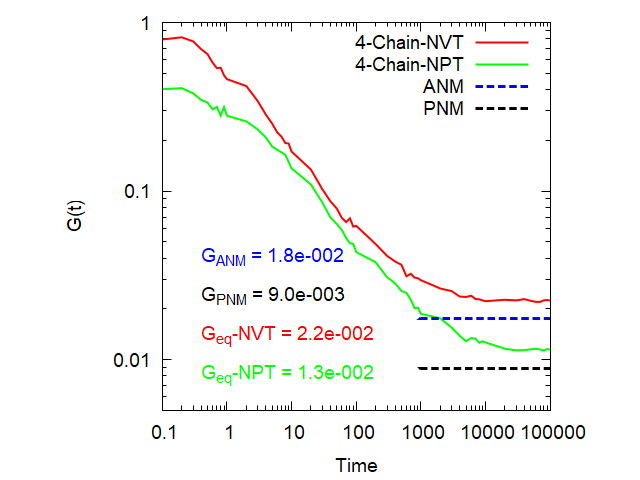
\includegraphics[width=\textwidth]{gt_4chain_comp.png}
					% \includegraphics<2>[width=\textwidth]{gt_NPT_mod.png}
				\end{block}
		\end{columns}
\end{frame}

\begin{frame}
    \frametitle{Z1-code での確認}
    \vspace{-3mm}
        \begin{columns}[T, onlytextwidth]
            \column{.42\linewidth}
            \vspace{-3mm}
            \begin{center}
                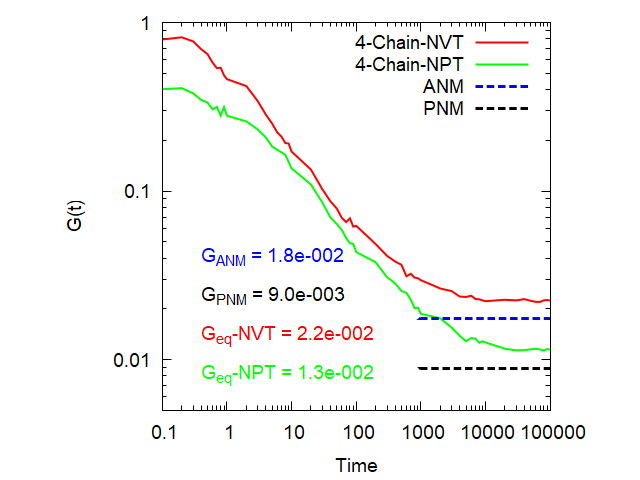
\includegraphics[width=\textwidth]{gt_4chain_comp.png}
                
                \vspace{3mm}
                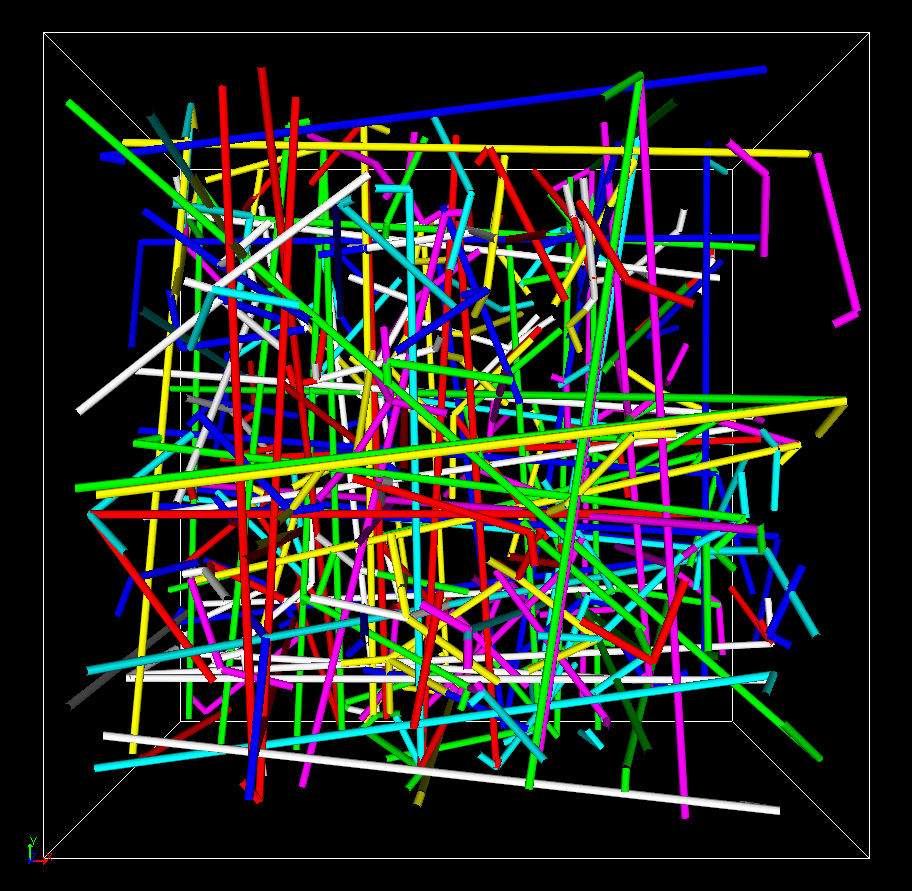
\includegraphics[width=.7\textwidth]{z_cord_NPT_4Chain.png}

                \scriptsize
                Z1-code for NPT
            \end{center}
            \column{.55\linewidth}
            \begin{block}{絡み合いの効果}
                \begin{itemize}
                    \item 一つの絡み合いごとに、\\ストランド数増加と仮定。
                    \item NPT計算では絡み合いで、説明可能。
                \end{itemize}

                \vspace{-3mm}
                \scriptsize
                \begin{center}
                    \begin{tabular}{c|c|c} \hline
                        &NPT & NVT \\ \hline \hline
                        \textcolor{blue}{Chains} & \multicolumn{2}{|c}{\textcolor{blue}{768}}\\ \hline
                        \textcolor{blue}{$\nu_0$}& \multicolumn{2}{|c}{\textcolor{blue}{0.018}}\\ \hline
                        \textcolor{blue}{$G_0 = \nu_0\times (1-2/4)$}&\multicolumn{2}{|c}{\textcolor{blue}{0.009}} \\ \hline \hline
                        Entanglements& 278& 800\\ \hline
                        Entangled Chains&249&557 \\ \hline
                        \alert{$\nu$}& \alert{0.024}&\alert{0.036}\\ \hline
                        $\nu/\nu_0$& 1.4& 2.0 \\ \hline
                        $G_{calcd.}=G_0 \times \nu/\nu_0$ & \alert{0.012} & 0.018 \\ \hline \hline
                        $G_{measd.}$ & \alert{0.013} & 0.022 \\ \hline
                    \end{tabular}
                \end{center}
            \end{block}
        \end{columns}
\end{frame}

\begin{frame}
    \frametitle{Rubinstein の先行研究}
        \begin{center}
            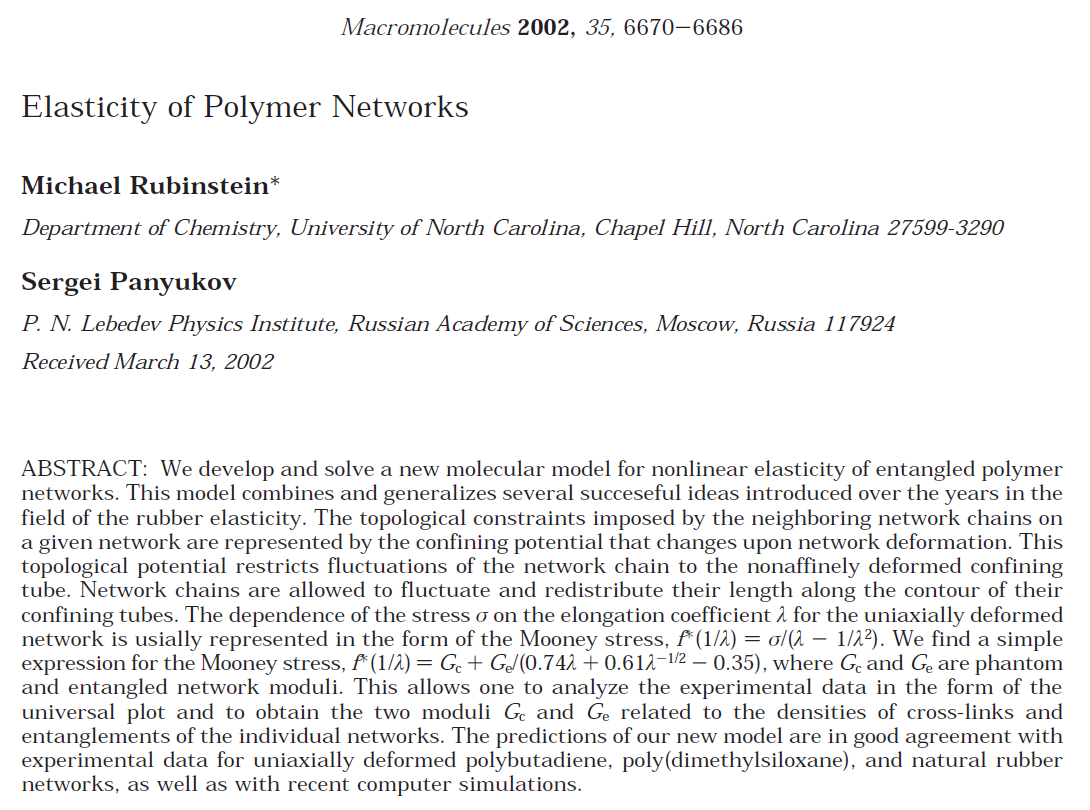
\includegraphics[width=.8\textwidth]{./rubinstein_1.png}
        \end{center}
\end{frame}

\begin{frame}
    \frametitle{Rubinstein の先行研究}

        この論文は、難解で全然読めていないのですが、増渕先生に以下の部分だけを紹介してもらって、まずの見積もりをしました。

        本当は、アブストラクトに書いてある、絡み合いの緩和のほうが重要なんですが、そこまではできていません。

        \begin{center}
            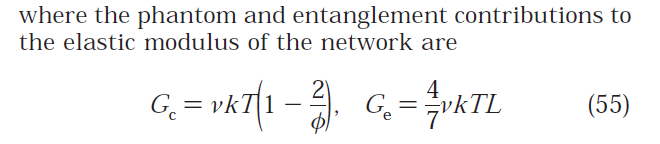
\includegraphics[width=.8\textwidth]{./rubinstein_2.png}

            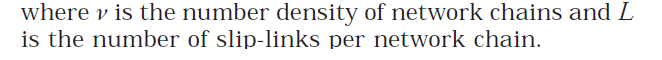
\includegraphics[width=.8\textwidth]{./rubinstein_3.png}
        \end{center}
\end{frame}

\begin{frame}
    \frametitle{絡み合いの効果について}
    \vspace{-3mm}
        % \begin{columns}[T, onlytextwidth]
        %     \column{.55\linewidth}
        %     \begin{block}{絡み合いの効果}
            \small
                \begin{itemize}
                    \item ストランドごとの絡み合いが少なければほぼ一致。
                    \item 絡み合いが増えると、ガウス鎖として振る舞うという仮定からずれて、寄与の因子が4/7よりも増加?
                \end{itemize}

                % \vspace{-3mm}
                % \scriptsize
                \begin{center}
                    \begin{tabular}{c|c|c} \hline
                        &NPT & NVT \\ \hline \hline
                        \textcolor{blue}{Chains} & \multicolumn{2}{|c}{\textcolor{blue}{768}}\\ \hline
                        \textcolor{blue}{$\nu$}& \multicolumn{2}{|c}{\textcolor{blue}{0.018}}\\ \hline
                        \textcolor{blue}{$G_c = \nu \times (1-2/4)$}&\multicolumn{2}{|c}{\textcolor{blue}{0.009}} \\ \hline \hline
                        Entanglements& 278& 800\\ \hline
                        Entangled Chains&249&557 \\ \hline
                        L & 278/768=0.36 & 800/768=1.04 \\ \hline
                        $G_e=4/7 \times \nu \times L $ & 0.004 & 0.011 \\ \hline \hline
                        $G_{calcd.}=G_c + G_e$ & 0.013 & 0.020 \\ \hline \hline
                        $G_{measd.}$ & 0.013 & 0.022 \\ \hline
                    \end{tabular}
                \end{center}
        %     \end{block}
        %     \column{.42\linewidth}
        %     \vspace{-3mm}
        %     \begin{center}
        %         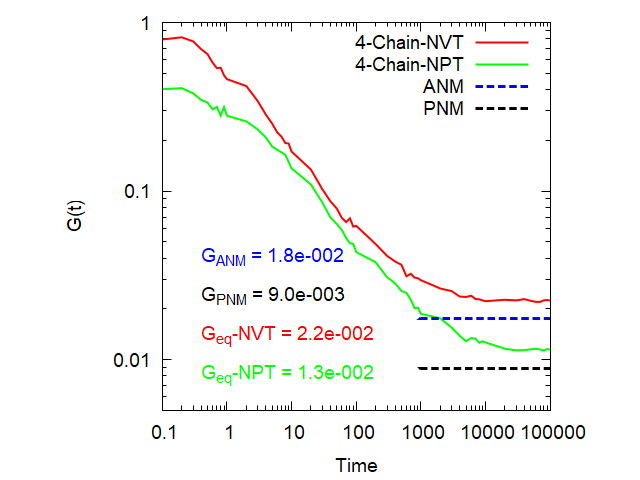
\includegraphics[width=\textwidth]{gt_4chain_comp.png}
                
        %         \vspace{3mm}
        %         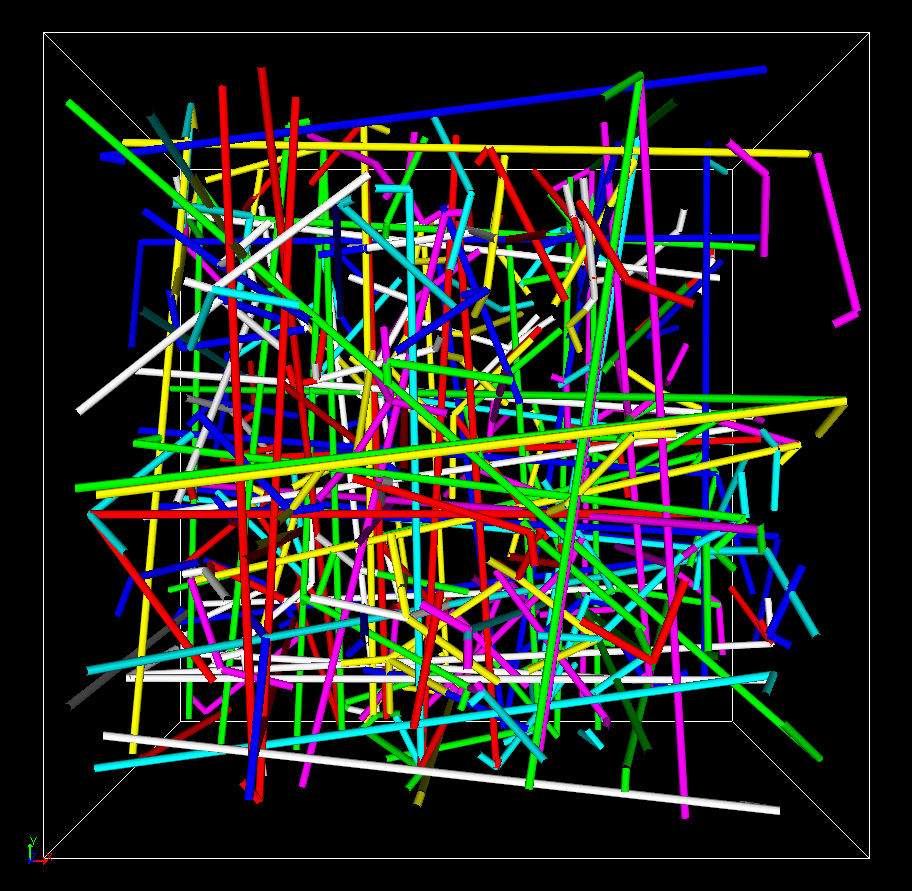
\includegraphics[width=.7\textwidth]{z_cord_NPT_4Chain.png}

        %         \scriptsize
        %         Z1-code for NPT
        %     \end{center}
        % \end{columns}
\end{frame}

\begin{frame}
    \frametitle{ヒステリシスの検討}
        \begin{block}{計算条件}
            \begin{itemize}
                \item 変形:へンキーひずみ
                \item 伸張速度:$\dot{\lambda} = 1E-4 [1/\tau]$
            \end{itemize}
        \end{block}
    \begin{columns}[T, onlytextwidth]
        \column{.48\linewidth}
        \begin{itemize}
            \item 4-Chain-NVT
        \end{itemize}
            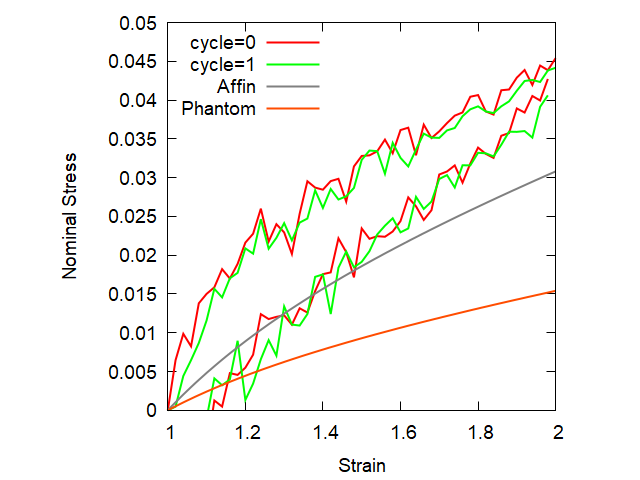
\includegraphics[width= \textwidth]{hyst_4Chain.png}
        \column{.48\linewidth}
        \begin{itemize}
            \item 4-Chain-NPT
        \end{itemize}
            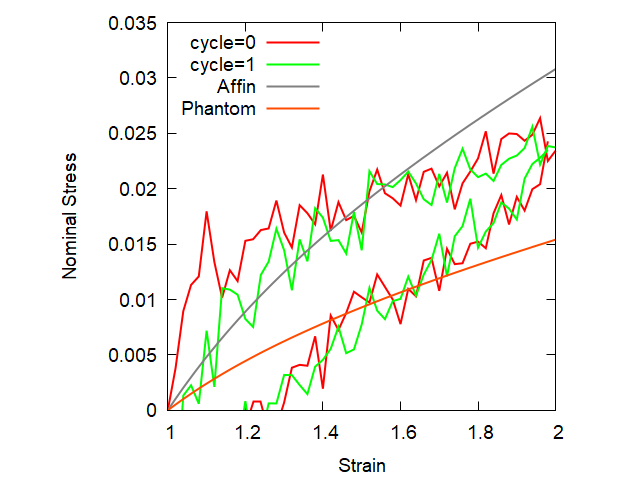
\includegraphics[width=\textwidth]{hyst_NPT_4Chain.png}
    \end{columns}
\end{frame}

\begin{frame}
	\frametitle{おわりに}
		\begin{block}{本発表の内容}
			\begin{itemize}
			\item ネットワーク構造の連結性にランダム性を導入
				\begin{itemize}
					\item 各ノードごとにランダムな結合性を導入
					\item ストランドの末端間距離がガウス分布する\\ランダムネットワーク構造
				\end{itemize}
			\item ランダムネットワーク構造の力学的応答
				\begin{itemize}
					\item 比較的長時間での緩和を確認
					\item Trapped Entanglements が緩和後の弾性率に影響 
					\item ファントムネットワークモデルの挙動を確認
				\end{itemize}
			\end{itemize}
		\end{block}
\end{frame}


% %%%%%%%%%%%%%%%%%%%%%%%%%%%%%%%%%%%%%%%%%%%%%%%
% \appendix
% \backupbegin

% %%%%%%%%%%%%%%%%
% \begin{frame}
% 	\LARGE{補足資料}
% \end{frame}
% %%%%%%%%%%%%%%%

% % \section{補足}

% \begin{frame}
%     \frametitle{規則ネットワークのヒステリシス}
%         \begin{block}{計算条件}
%             \begin{itemize}
%                 \item 変形:へンキーひずみ
%                 \item 伸張速度:$\dot{\lambda} = 1E-4 [1/\tau]$
%             \end{itemize}
%         \end{block}
%         \begin{center}
%             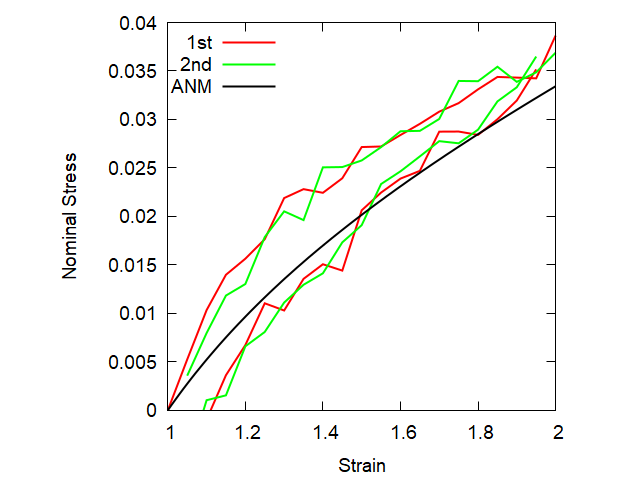
\includegraphics[width=.6\textwidth]{hyst_4chain_reg.png}
%         \end{center}
% \end{frame}

% \begin{frame}
% 	\frametitle{「す抜け鎖」での一軸伸長}
% 		\begin{exampleblock}{一軸伸長:Z軸方向に二倍に伸長}
% 			\begin{itemize}
% 				\item ストランド:す抜け鎖
% 				\item 四分岐ランダムネットワークモデル
% 				\item 初期長さ:$|\bm{R_z}| = 3.46$
% 				\item 伸長後:$|\bm{R_z}| = 5.62 \Leftarrow$ \alert{二倍には伸びていない}
% 			\end{itemize}
% 		\end{exampleblock}
% 		\begin{columns}[totalwidth=\linewidth]
% 			\column{.48\linewidth}
% 				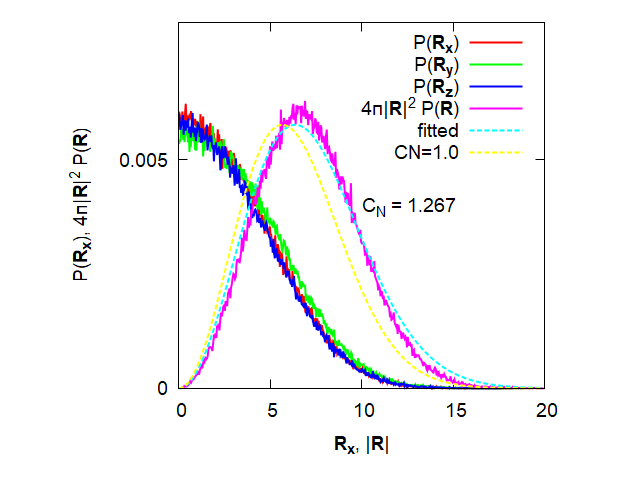
\includegraphics[width=1.1\columnwidth]{4chain_E2E_init.png}
% 			\column{.48\linewidth}
% 				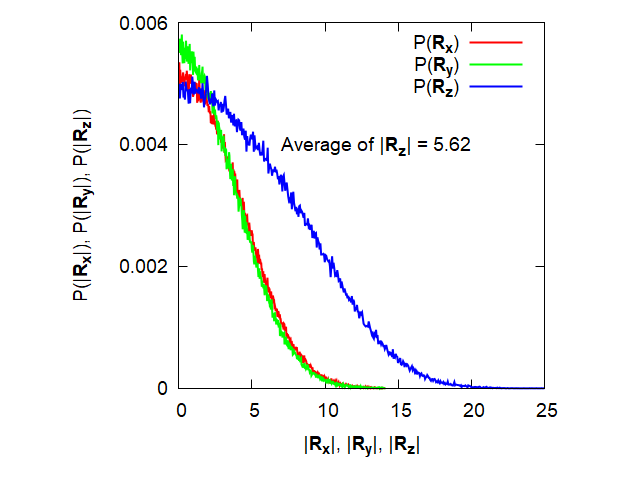
\includegraphics[width=1.1\columnwidth]{Expand_4_Strand_histgram.png}
% 		\end{columns}
% \end{frame}

% \begin{frame}
% 	\frametitle{四分岐ネットワークの平衡構造}
% 		\begin{columns}[T, onlytextwidth]
% 			\column{.48\linewidth}
% 				\begin{block}{四分岐ネットワークの作成}
% 					\begin{itemize}
% 						\item ストランドの末端間距離がホモポリマーと同等となるように、
% 						\item セグメント数 N=48 のストランドを選択し、
% 						\item 多重度を 3 とした四分岐ネットワークを作成。
% 						% \item 十分に初期緩和
% 					\end{itemize}
% 					\begin{center}
% 						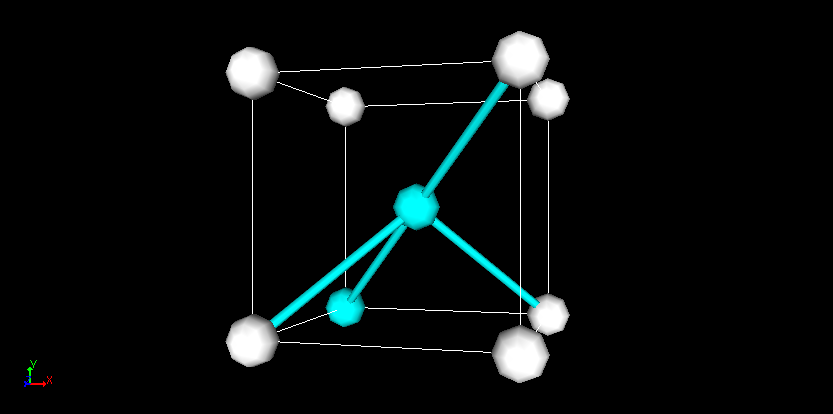
\includegraphics[width=.6\textwidth]{8_4.png}
% 					\end{center}
% 				\end{block}
% 			\column{.5\linewidth}
% 				\footnotesize
% 				\begin{itemize}
% 					\item 鎖に沿ったセグメント間\\距離のトラジェクトリ
					
% 					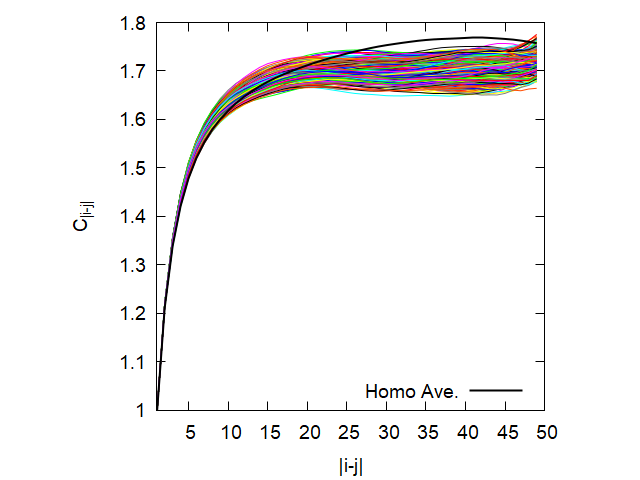
\includegraphics[width=.64\textwidth]{N48_f4_CN.png}

% 					\item 末端間距離の分布関数
					
% 					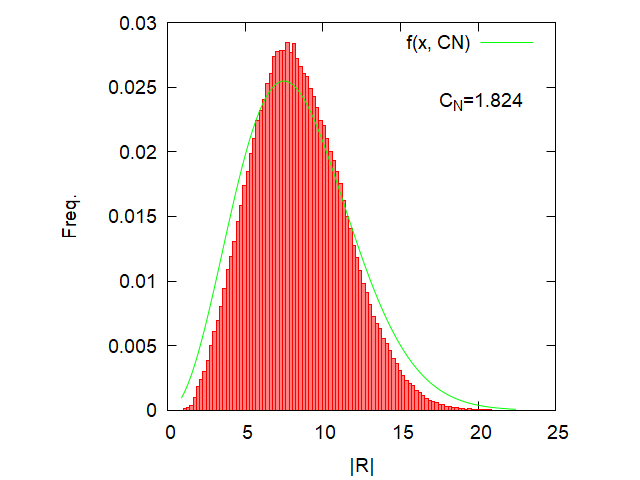
\includegraphics[width=.64\textwidth]{R_N48_f4.png}
% 				\end{itemize}
% 		\end{columns}
% \end{frame}

% \begin{frame}
% 	\frametitle{ネットワーク構造でのG1-cord}
% 		\begin{center}
% 			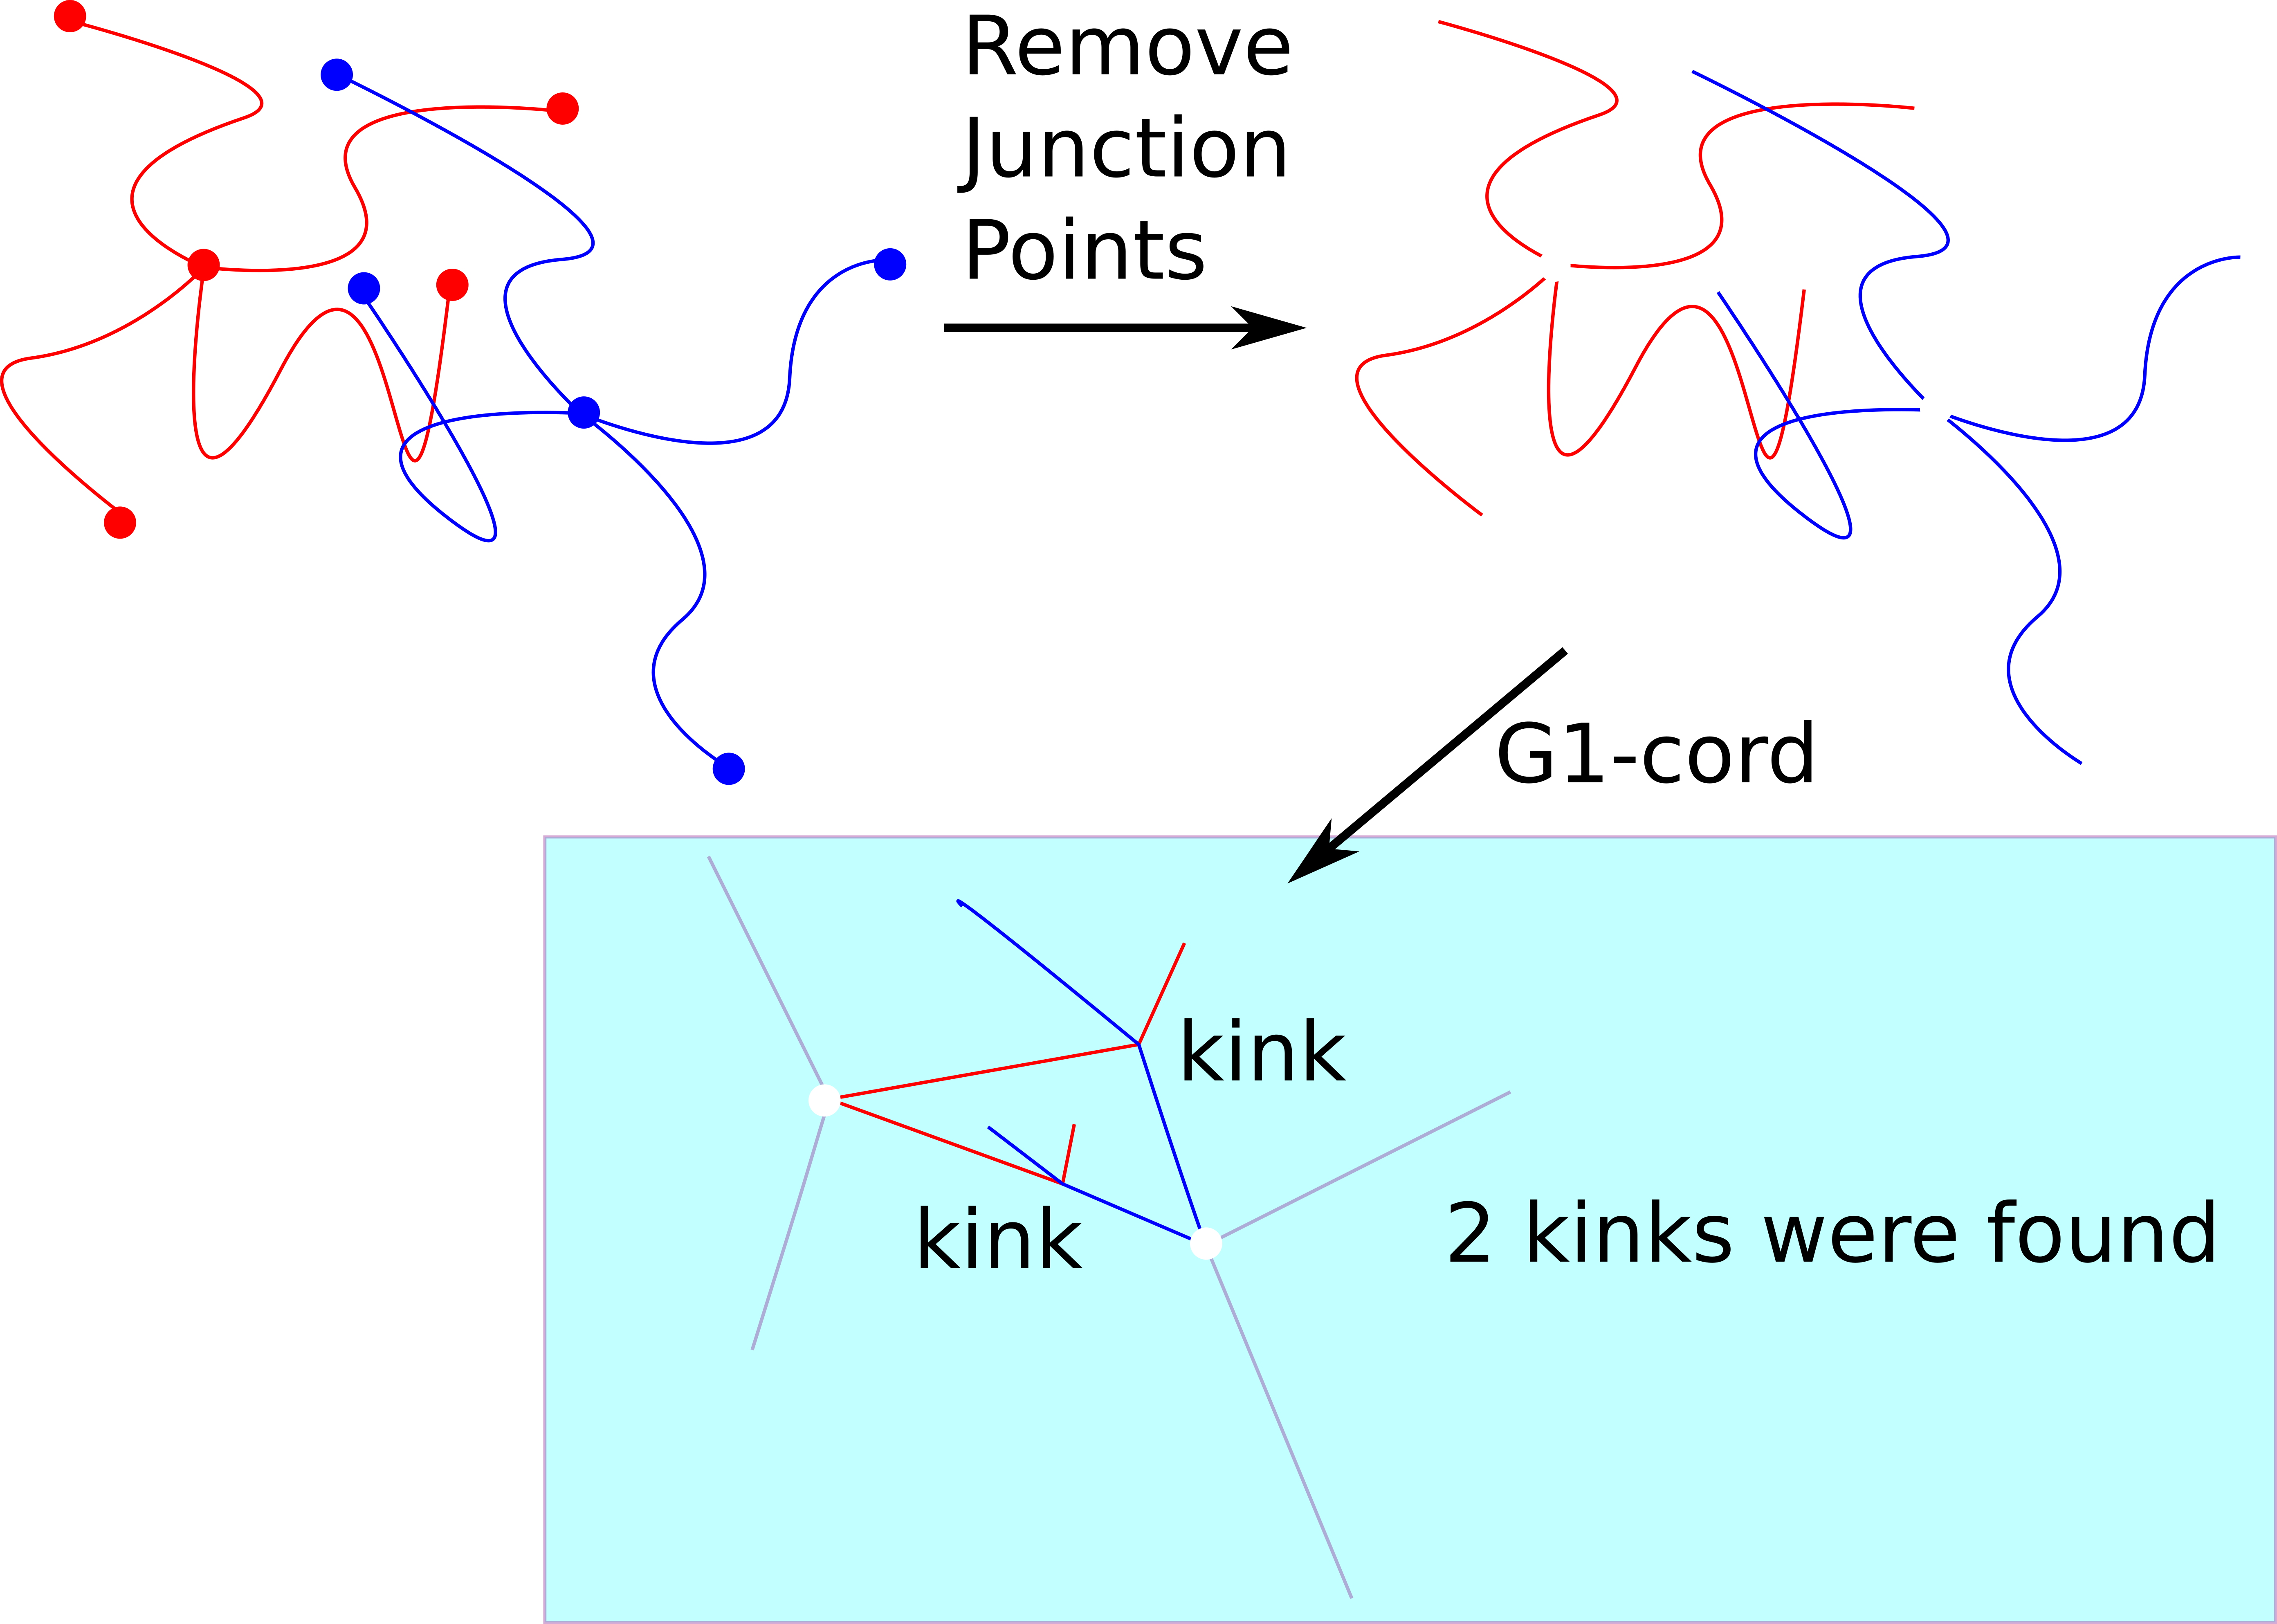
\includegraphics[width=.8\textwidth]{g1cord.png}
% 		\end{center}
% \end{frame}

% \section{ランダムネットワークの作成}

% \subsection{ランダムネットワークの作成}
% \begin{frame}
% 	\frametitle{トポロジーモデルへの変換}
% 		\begin{columns}[totalwidth=\textwidth]
% 			\column{.48\textwidth}
% 				\begin{block}{実空間での初期構造}
% 					\begin{itemize}
% 						\item $2\times2\times2$ 個の\\ユニットセル
			
% 							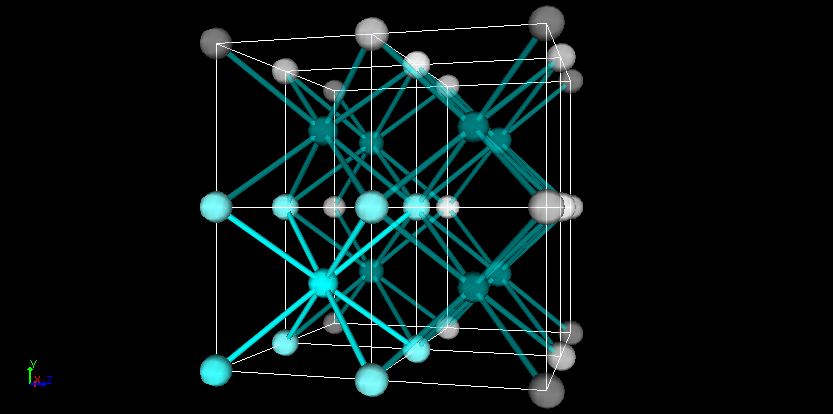
\includegraphics[width=0.8\columnwidth]{8_per.png}

% 						\item ユニットセルから除去

% 							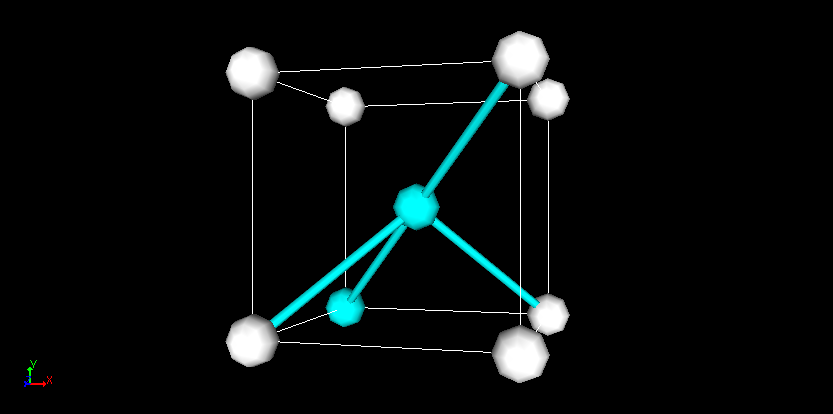
\includegraphics[width=0.8\columnwidth]{8_4.png}

% 					\end{itemize}
% 				\end{block}
% 		\column{.48\textwidth}
% 			\begin{exampleblock}{トポロジーモデル}
% 				分岐数を4に減じた\\トポロジーモデル

% 				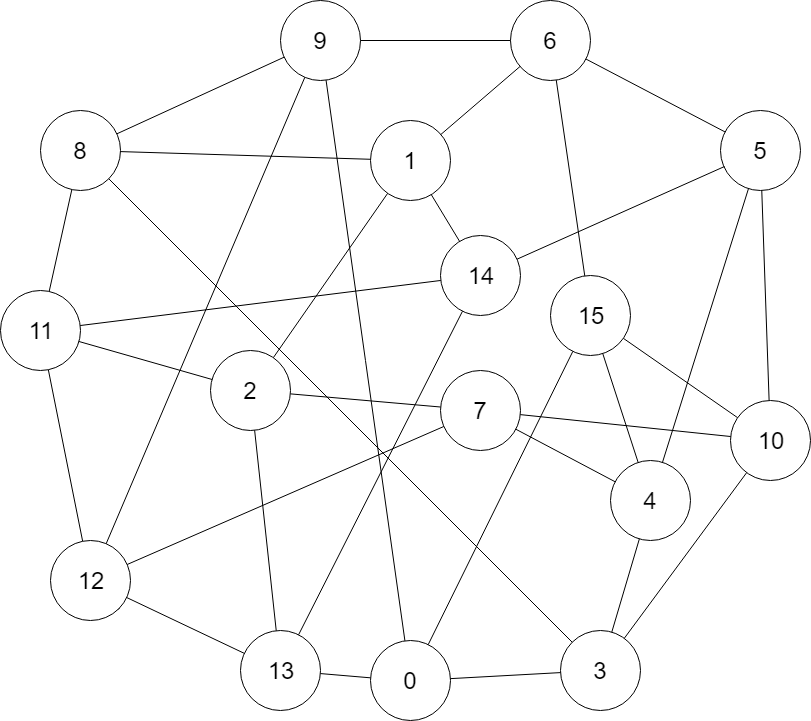
\includegraphics[width=\columnwidth]{Network.png}

% 			\end{exampleblock}
% 		\end{columns}
% \end{frame}

% \begin{frame}
% 	\frametitle{それぞれの分岐数での初期構造}
% 		\begin{exampleblock}{初期構造の作成}
% 			\begin{itemize}
% 				\item \alert{実空間}で8-Chain Model で初期構造を作成。
% 				\item 所望の分岐数に\alert{ランダム}に選択した\alert{結合を除去}
% 				\item 除去したジオメトリーに対応した\alert{トポロジーモデル}
% 			\end{itemize}
% 		\end{exampleblock}
% 		\begin{columns}[totalwidth=\linewidth]
% 			\column{.48\linewidth}
% 				\begin{block}{分岐数: 3, 4, 5 分岐}
% 					\begin{itemize}
% 						\item 3 分岐では、全てが連結していない
% 						\item 4 分岐では、連結していないものもある
% 						\item 5 分岐でも二種類のみ
% 					\end{itemize}
% 				\end{block}
% 			\column{.48\linewidth}
% 				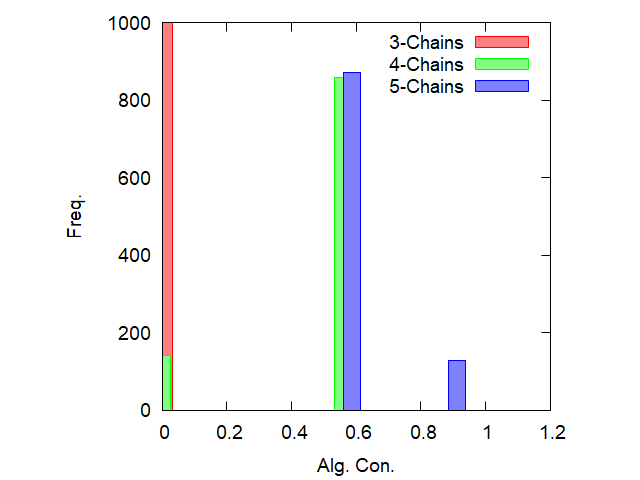
\includegraphics[width=\columnwidth]{Histgram2.png}
% 		\end{columns}
% \end{frame}

% \begin{frame}
% 	\frametitle{トポロジーモデルからのランダム性の導入}
% 		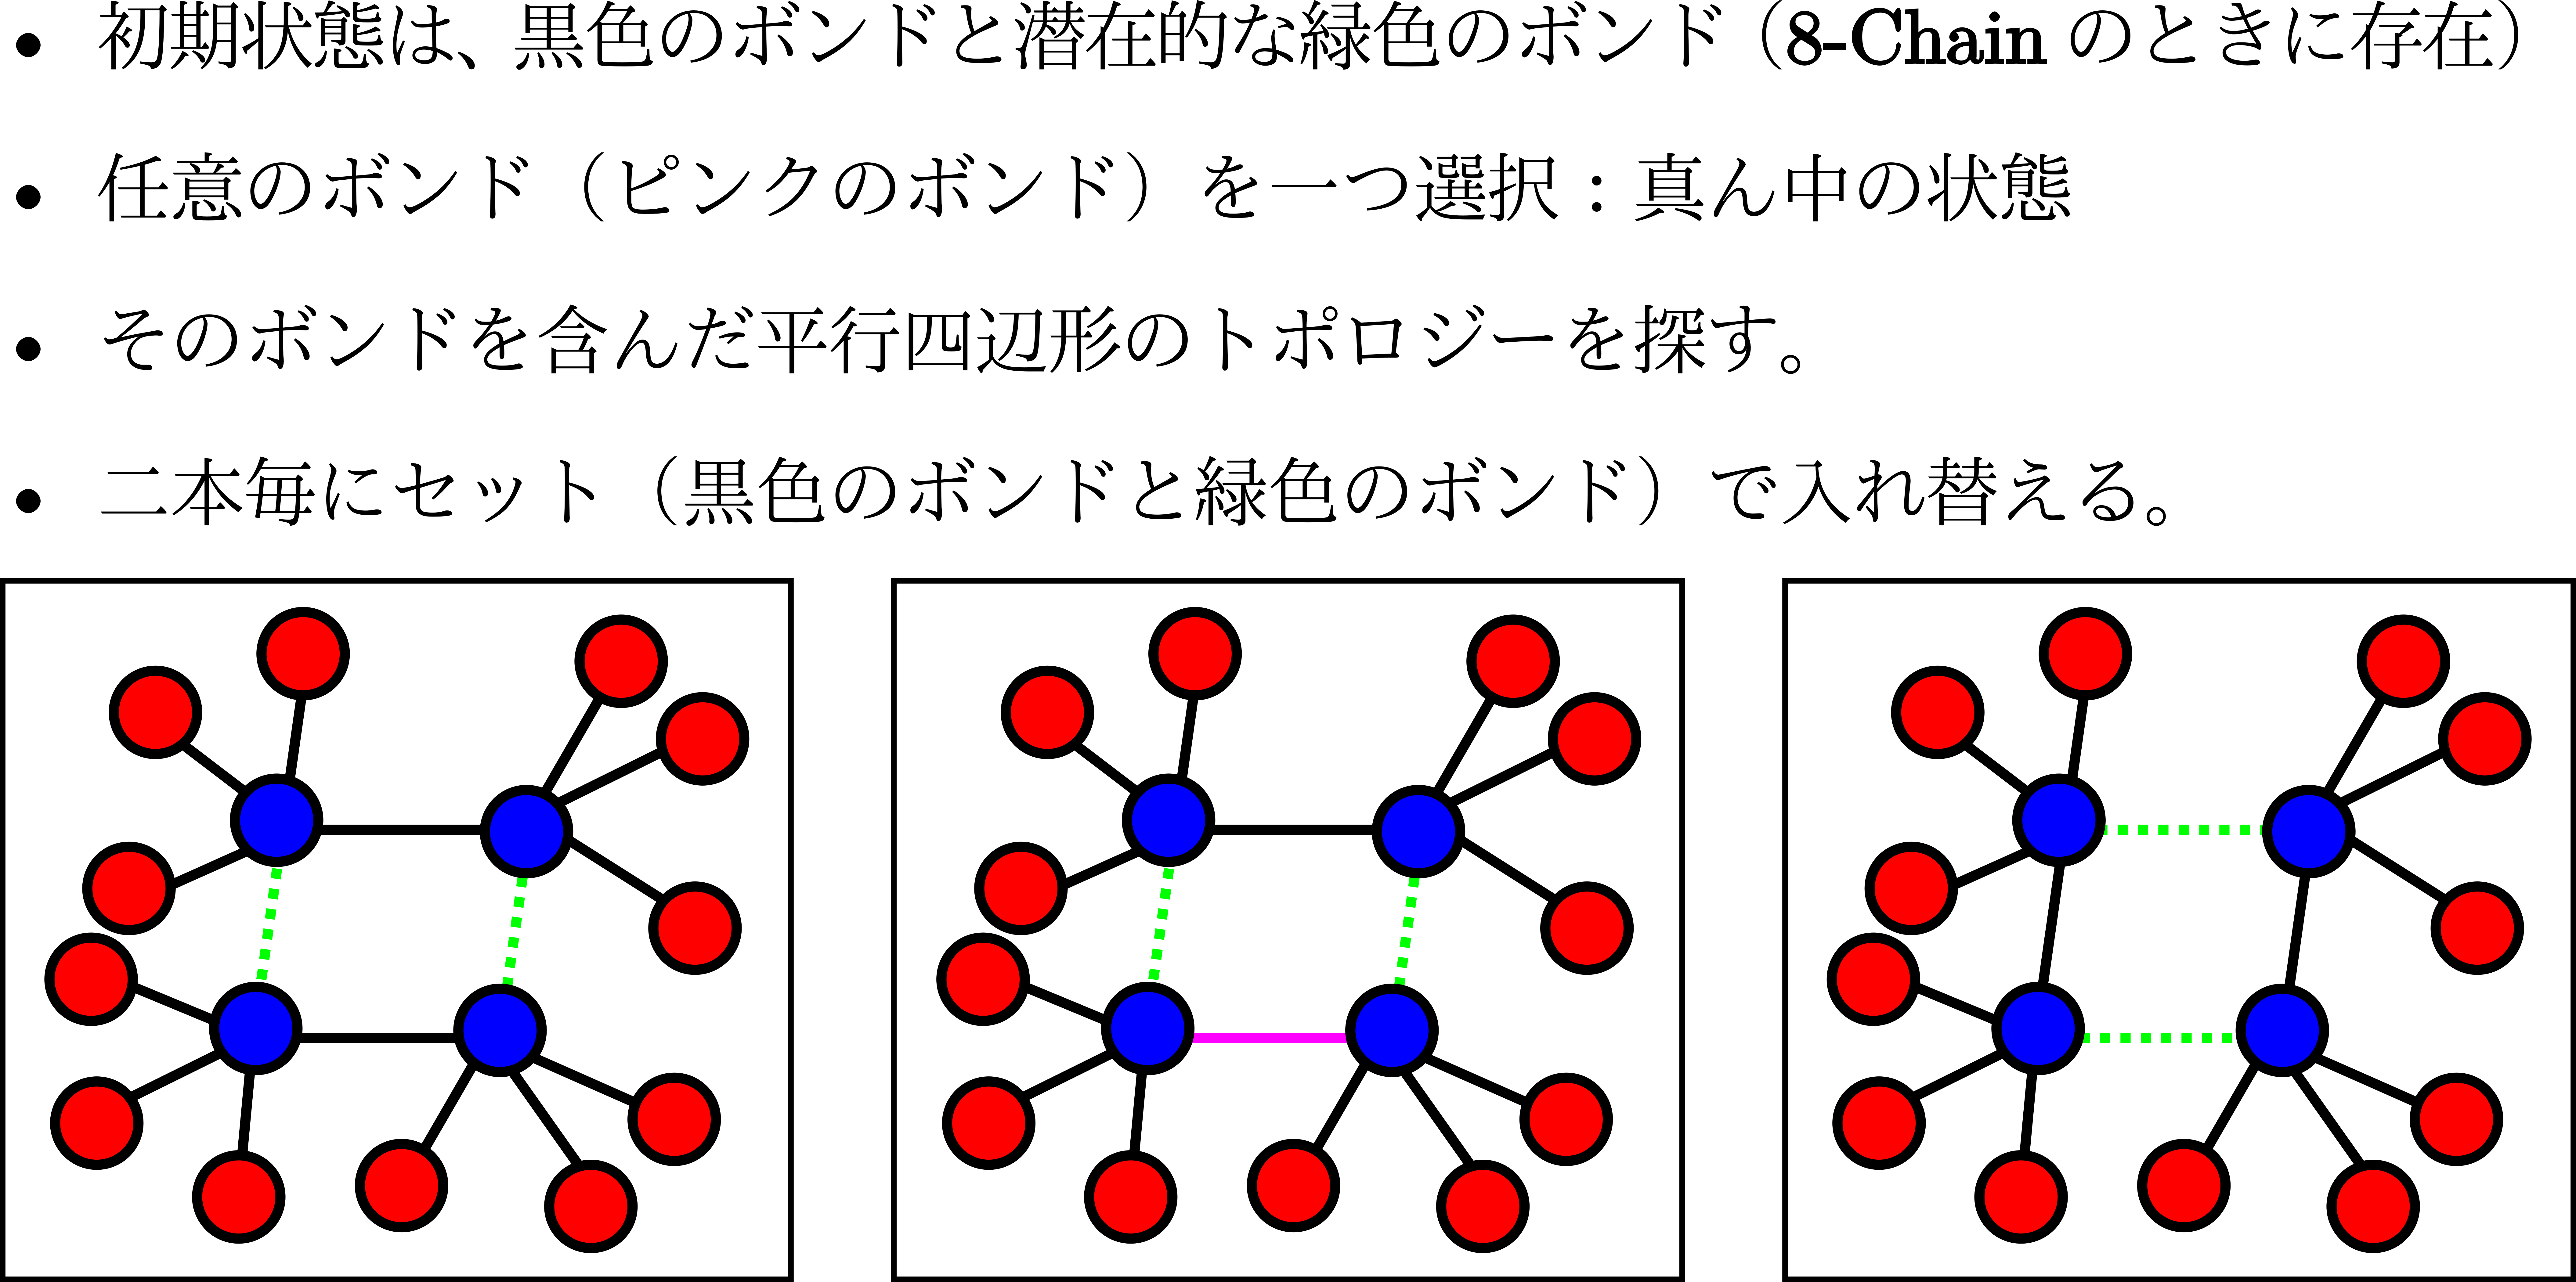
\includegraphics[width=\textwidth]{bond_exchg.png}
% \end{frame}

% \begin{frame}
% 	\frametitle{代数的連結性の分布関数}
% 		\begin{exampleblock}{サンプリング数の増加($> 1000,000$ times)}
% 			\begin{itemize}
% 				\item 3, 5分岐トポロジーモデルは、単鋒性に
% 				\item 4分岐のトポロジーモデルでは、二峰性\\
% 				サンプリング数を増やすと若干変化
% 			\end{itemize}
% 		\end{exampleblock}
% 		\begin{columns}[totalwidth=1\textwidth]
% 			\column{.33\textwidth}
% 				\begin{center}
% 					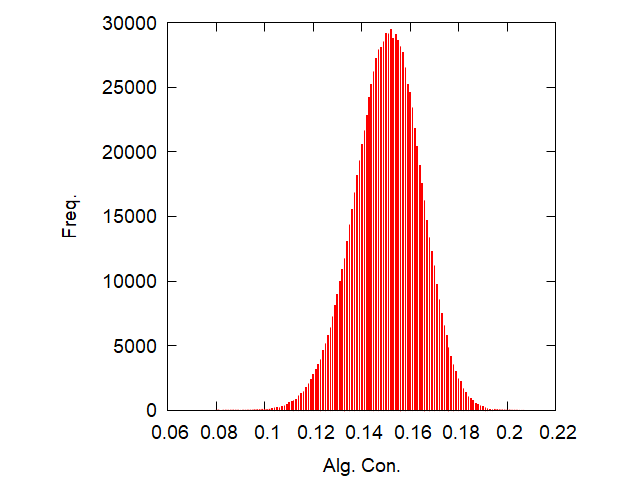
\includegraphics[width=1.2\columnwidth]{3.png}

% 					3-Chain Model
% 				\end{center}
% 			\column{.33\textwidth}
% 				\begin{center}
% 					\includegraphics[width=1.2\columnwidth]{4_1000_5000.png}

% 					4-Chain Model
% 				\end{center}
% 			\column{.33\textwidth}
% 				\begin{center}
% 					\includegraphics[width=1.2\columnwidth]{5.png}

% 					5-Chain Model
% 				\end{center}
% 		\end{columns}
% \end{frame}


% \subsection{ネットワークのトポロジー}
% \begin{frame}
% 	\frametitle{ネットワークの分岐数の処理}
% 		以下のようにノード番号を付与したネットワークを考えると、
% 			\begin{center}
% 				\includegraphics[width=4cm]{NW-4.png}
% 			\end{center}
% 		隣接行列、および、次数行列は、
% 		\begin{align*}
% 			A = \left( 
% 			\begin{array}{cccc} 
% 			0 & 1 & 1 & 1 \\ 
% 			1 & 0 & 1 & 0 \\
% 			1 & 1 & 0 & 1 \\
% 			1 & 0 & 1 & 0 
% 			\end{array} 
% 			\right) 
% 			,
% 			D = \left( 
% 			\begin{array}{cccc} 
% 			3 & 0 & 0 & 0 \\ 
% 			0 & 2 & 0 & 0 \\
% 			0 & 0 & 3 & 0 \\
% 			0 & 0 & 0 & 2 
% 			\end{array} 
% 			\right) 
% 		\end{align*}
% 		となる。
% \end{frame}

% \subsection{ラプラシアン行列}
% \begin{frame}
% 	\frametitle{ラプラシアン行列}
% 		\begin{columns}[totalwidth=1\textwidth]
% 			\column{.48\textwidth}
% 				ラプラシアン行列は、隣接行列$A$と次数行列$D$により以下のように定義される。
% 				$$
% 				L \equiv D-A
% 				$$
% 				4つのノードからなるネットワークの例であれば、
% 				$$
% 				L = \left( 
% 				\begin{array}{cccc} 
% 				3 & -1 & -1 & -1 \\ 
% 				-1 &  2 & -1 & 0 \\
% 				-1 & -1 &  3 & -1 \\
% 				-1 &  0 & -1 & 2 
% 				\end{array} 
% 				\right) 
% 				$$
% 				となり、非負の固有値。
% 			\column{.48\textwidth}
% 				グラフが非連結であるとき、%ラプラシアン行列の成分を
% 				連結した成分ごとにブロック対角化できるので、固有値 0 の重複数がグラフの連結成分ブロックの総数となる。
% 				\begin{block}{「代数的連結性」}
% 					「グラフが連結である場合、ラプラシアン行列の固有値 0 の重複数は 1」となる。\\
% 					固有値を昇順にみた時、0 に次ぐ二番目の固有値がグラフの連結性の強さを示す指標となり、「代数的連結性」と呼ばれる。
% 				\end{block}
% 		\end{columns}
% \end{frame}

% \section{ファントムネットワークの理論}
% \subsection{ファントムネットワークの理論}
% \begin{frame}
% 	\frametitle{有限サイズ効果}
% 		\begin{columns}[totalwidth=1\textwidth]
% 			\column{.48\textwidth}
% 				\begin{block}{末端の壁面固定の効果}
% 				\begin{itemize}
% 					\item 壁面に末端が固定
% 						\begin{itemize}
% 							\item $n$ 本のストランド
% 							\item セグメント数: $N$
% 							\item 他端が架橋点($\bm{r}$)
% 						\end{itemize}
% 					\item 架橋点の運動性
% 						\begin{itemize}
% 							\item 壁と$N/n$ 個の短い\\ストランドと等価
% 							\item 壁の移動(変形)の影響減少
% 						\end{itemize}
% 				\end{itemize}
% 				% \vspace{-2mm}
% 				\begin{center}
% 					\includegraphics[width=.8\textwidth]{phantom-1.png}
% 				\end{center}
% 				\end{block}
% 			\column{.48\textwidth}
% 				\begin{exampleblock}{内部の鎖が受ける変形}
% 					\begin{itemize}
% 						\item システム内部の鎖の末端はガウス分布
% 						\item 壁面固定の末端からの変形が内部に伝達して、
% 					\end{itemize}
% 					\vspace{-3mm}
% 					\tiny
% 					\begin{align*}
% 						&G=\xi \nu k_BT \\
% 							&\begin{cases}
% 							\xi_{\infty} = 1-\dfrac{2}{f} \;\; \text{System}\sim \infty \\[8pt]
% 							\xi_{s} = \dfrac{f-1}{f+1} \;\; \text{Small Limit}
% 							\end{cases}
% 					\end{align*}
% 					\vspace{-5mm}
% 					\begin{center}
% 						\includegraphics[width=0.5\textwidth]{phantom.png}
% 					\end{center}
% 				\end{exampleblock}
% 		\end{columns}
% \end{frame}
% %%%%%%%%%%%%%%%%%%%%%%%%%%

% %%%%%%%%%%%%%%%%%%%%%%%%%%%%%%%%%%%%%%%%%%%%%%
% \subsection{ファントムネットワークの振る舞い}
% \begin{frame}
% 	\frametitle{ファントムネットワークのゆらぎ}
% 		\begin{block}{ゆらぎの入ったポテンシャル}
% 			\begin{itemize}
% 				\item ストランドの末端間ベクトル $\bm{R}_{nm}$ を、\\架橋点の位置ベクトル $\bm{r}_n$ を用いて、
% 					\footnotesize
% 					\begin{equation*}
% 						\bm{R}_{nm} \equiv \bm{r}_n-\bm{r}_m
% 					\end{equation*}
% 					\normalsize
% 				\item 系のポテンシャルエネルギーは、
% 					\footnotesize
% 					\begin{equation*}
% 						U=\dfrac{k}{2} \sum_{\langle nm \rangle} \bm{R}_{nm}^2
% 					\end{equation*}
% 					\normalsize
% 				\item これは、自然長で決まる定数項と、ゆらぎに起因した第二項に分割でき、その和で以下となる。
% 					\footnotesize
% 					\begin{equation*}
% 						U=\dfrac{k}{2} \sum_{\langle nm \rangle} {\bm{R}_{nm}^{(0)}}^2 + \dfrac{k}{2} \sum_{\langle nm \rangle} \Delta \bm{R}_{nm}^2
% 					\end{equation*}
% 					\normalsize
% 			\end{itemize}
% 		\end{block}
% \end{frame}

% \begin{frame}
% 	\frametitle{ファントムネットワークのゆらぎ}
% 		\begin{block}{アンサンブル平均の二つの表式}
% 			\vspace{-5mm}
% 			\scriptsize
% 			\begin{align*}
% 				\begin{cases}
% 					\langle U \rangle = N_{strands} \dfrac{k}{2} \langle \Delta \bm{R}^2 \rangle \\
% 					\langle U \rangle = 3(N_{nodes}-1) \dfrac{1}{2} k_B T
% 				\end{cases}
% 			\end{align*}
% 			\normalsize
% 			なお、第二式は等分配側より導出した。
% 		\end{block}
% 		\begin{exampleblock}{ファントムネットワークでのゆらぎ}
% 			\begin{itemize}
% 				\item 架橋点数 $N_{nodes}$、架橋点官能基数 $f$ とすれば、
% 					\scriptsize
% 					\begin{equation*}
% 					\langle \Delta \bm{R}^2 \rangle = \dfrac{3k_B T}{k} \dfrac{2}{f} \left( 1-\dfrac{1}{N_{nodes}} \right)
% 					\end{equation*}
% 					\normalsize
% 				\item 適切な条件で、ストランドの自然長 $R_0$ を用いて、
% 					\scriptsize
% 					\begin{equation*}
% 					\color{red}
% 					\langle \Delta \bm{R}^2 \rangle = \dfrac{2}{f} R_0^2
% 					\end{equation*}
% 					\normalsize
% 			\end{itemize}
% 		\end{exampleblock}
% \end{frame}

% %%%%%%%%%%%%%%%%%%%%%%%%%%%%
% \section{その他}
% \subsection{破壊について}
% \begin{frame}
% 	\frametitle{高分子材料への期待と不安}
% 	地球温暖化対策の CO$_2$ 削減へ向けて、\\
% 	{\color{red}「自動車を中心とした運送機器の抜本的な軽量化」}
% 	\\
% 	が提唱されている。
% 	\begin{block}{高分子材料への期待}
% 		\begin{itemize}
% 			\item 現行の鉄鋼主体$ \Rightarrow$ 高分子材料を含むマルチマテリアル化
% 			\item 高分子材料によるマルチマテリアル化のポイント
% 				\begin{itemize}
% 					\item 高い比強度の有効利用
% 					\item 特徴を生かした適材適所 $\Leftrightarrow$ 適切な接合方法の選択
% 						\begin{itemize}
% 							\item {\color{red} 「接着接合」への高分子の利用}
% 							\item {\color{red} 「柔らかさを生かした弾性接着接合」}
% 						\end{itemize}
% 					\item {\color{blue}耐久性が不明確(特に疲労破壊に対して)}
% 				\end{itemize}
% 		\end{itemize}
% 	\end{block}
% \end{frame}

% %%%%%%%%%%%%%%%%%%%%%%%%%%%%%%
% \begin{frame}
% 	\frametitle{破壊工学の考え方}
% 		\begin{exampleblock}{破壊工学の考え方}
% 			\begin{itemize}
% 				\item 系中のクラック存在を前提に材料の耐久性を評価
% 				\item \alert{「クラック近傍の応力集中を如何に抑制?」}がポイント
% 			\end{itemize}
% 		\end{exampleblock}
% 		\begin{columns}[totalwidth=1\textwidth]
% 			\column{.5\textwidth}
% 				\begin{alertblock}{破壊工学の観点から(微視的)}
% 					\begin{itemize}
% 						\item クラック先端で応力集中\\ \alert{応力拡大係数 $K_I$ で評価}
% 							\footnotesize
% 							\begin{align*}
% 							K_{I} = \sigma \sqrt{\pi c}
% 							\end{align*}
% 							\normalsize
% 						\item クラック進展の抑制 \\
% 							$\Rightarrow$ 
% 							% 先端での\alert{局所降伏}\\
% 							降伏応力 $\sigma_Y$ に反比例
% 							\footnotesize
% 							\begin{align*}
% 							d \propto \left( \dfrac{K_I}{\sigma_Y} \right)^2
% 							\end{align*}
% 							\normalsize
% 					\end{itemize}
% 				\end{alertblock}
% 		\column{.45\textwidth}
% 			\includegraphics[width=.9\textwidth]{Crack_Yield.pdf}
% 		\end{columns}
% \end{frame}

% \subsection{破壊と粘弾性}
% \begin{frame}
% 	\frametitle{ゴムの強靭性}
% 		\begin{columns}[totalwidth=\textwidth]
% 			\column{.62\textwidth}
% 				\begin{exampleblock}{Andrews 理論}
% 					クラック先端の応力の等高線表示
% 					\begin{itemize}
% 						\item クラック成長時の応力場の\\考察より、
% 							\begin{itemize}
% 								\item {\color{red} Loading 場とUnloading 場の差}が重要。
% 								\item この差は\alert{ヒステリシスに由来}
% 							\end{itemize}	
% 						\item \alert{ひずみエネルギー開放率が低減} \\$\Rightarrow$ 強靭さの起源。
% 					\end{itemize}
% 				\end{exampleblock}
% 				{Andrews, E. H. and Fukahori, Y., \\Journal of Materials Science, \\12, 1307 (1977)}
% 		\column{.35\textwidth}
% 			\includegraphics[width=\textwidth]{crack.png}
% 		\end{columns}
% \end{frame}

% \begin{frame}
% 	\frametitle{ゴムの破壊と粘弾性}
% 		\begin{alertblock}{ゴムの破壊}
% 			大変形を伴う非線形現象だが、時間温度換算則の成立が\\多数報告
% 		\end{alertblock}

% 		\begin{columns}[totalwidth=1\textwidth]
% 			\column{.48\textwidth}
% 				亀裂先端近傍での大変形
% 				\includegraphics[width=.7\textwidth]{rubber_crack.png}
% 			\column{.48\textwidth}
% 				時間温度換算則の成立
% 				\includegraphics[width=\textwidth]{Time_Temp_2.png}
% 				{\tiny Smith T., Stedry P., J. Appl. Phys. (1960) 31 1892}
% 		\end{columns}
% \end{frame}


% %%%%%%%%%%%%%%%%%
% \begin{frame}
% 	\frametitle{SBRでの伸びきり効果}
% 		\includegraphics[width=.8\textwidth]{SBR_lowTemp_2.png}

% 		{\footnotesize Smith TL., Dickie RA., J. Pol. Sci. part A-2 (1969) 7 635}
% 		\begin{alertblock}{室温で伸び切りが出ないはずのSBR}
% 			\begin{itemize}
% 				\item 低温、高速変形でSBRでも伸びきり効果が発現
% 				\item 時間温度換算則で考えてみれば?
% 			\end{itemize}
% 		\end{alertblock}
% \end{frame}

% \begin{frame}
% 	\frametitle{ガラス状態の高分子材料の疲労と破壊}
% 		\begin{columns}[totalwidth=1\textwidth]
% 			\column{.52\textwidth}
% 				\begin{block}{破壊のモード(巨視的)}
% 					脆性破壊 $\Leftrightarrow$ 延性破壊\\
% 					脆性破壊は、降伏前にミクロな\\クラックが進展した破壊
% 				\end{block}
% 			\column{.42\textwidth}
% 				\includegraphics[width=.8\textwidth]{S_S_Curve.png}
% 		\end{columns}
% 		\begin{exampleblock}{降伏と劣化}
% 			\begin{itemize}
% 				\item 靭性向上のため
% 				\begin{itemize}
% 					\item {\color{red} 局所的な降伏}が必須。\\(クレイズのような局所的な破壊も)
% 					\item 一般に、高分子材料の{\color{red} 降伏は不可逆}。
% 				\end{itemize}
% 				\item 降伏による劣化
% 					\begin{itemize}
% 						\item 降伏 $\Leftrightarrow$ {\color{red} 本質的には、少しずつ破壊。}
% 						\item {\color{red} 破壊領域への水分の浸透 $\Leftarrow$ 長期耐久性の欠如}
% 					\end{itemize}
% 			\end{itemize}
% 		\end{exampleblock}
% \end{frame}

% \subsection{ネットワークの振る舞い}
% \begin{frame}
% 	\frametitle{架橋点近傍の拘束状態に基づく二つのモデル}
% 		\begin{columns}[totalwidth=1\textwidth]
% 			\column{.45\textwidth}
% 				\begin{block}{ストランドと架橋点}
% 					\includegraphics[width=\textwidth]{JP_vicinity.png}
% 					架橋点はストランド経由で直接連結した架橋点以外の、近接する多数のストランド(図中の×)に囲まれている。
% 				\end{block}
% 			\column{.52\textwidth}
% 			\begin{itemize}
% 				\item ``Affine NW Model''\\
% 					架橋点は周辺に強く拘束され巨視的変形と相似に移動。(Affine 変形)
% 					\footnotesize
% 					\begin{align*}
% 						&G=\nu k_B T \\
% 						&\text{$\nu$ は、ストランドの数密度}
% 					\end{align*}
% 					\normalsize
% 				\item ``Phantom NW Model''\\
% 					架橋点が大きく揺らぎ、ずり弾性率($G$)が低下。
% 					\footnotesize
% 					\begin{align*}
% 						&G=\xi \nu k_B T \\
% 						&\xi= 1 -\dfrac{2}{f}\\
% 						&\text{$f$ は架橋点の分岐数}
% 					\end{align*}
% 			\end{itemize}
% 		\end{columns}
% \end{frame}

% \begin{frame}
% 	\frametitle{架橋点の近傍}
% 		\includegraphics[width=\textwidth]{Lake_Thomas.png}
% \end{frame}

% \backupend

\end{document}
